\chapter{Generalizando al sistema de Lotka-Volterra}

\section{Sistema de especies en competencia.}

\setlength{\parindent}{0cm} El sistema de Lotka-Volterra del que se ha hablado anteriormente es una de las grandiosas extensiones del \textit{modelo logístico} (\ref{eqn:EqLogistica}) que puede aplicarse a $N$ especies. En concreto, cuando es únicamente de competencia: las interacciones entre dichas especies son reales y positivas, y la dinámica se encuentra limitada por una o varias capacidades de carga.  Los términos no lineales de estas ecuaciones son cuadráticos y representan la relación entre la especie $i$ y la especie $j$. El conjunto de ecuaciones diferenciales que representa al sistema es el siguiente:
\begin{equation}\label{eqn:LK}
	\frac{dx_i}{dt}=r_ix_i\left(1-\frac{\sum_{j=1}^N \alpha_{ij}x_j}{K_i}\right)
\end{equation}
Donde $i,j\in\{1,...,N\}$, las ecuaciones consideran tasas de crecimiento $r_i$ y capacidades de carga $K_i$ que por lo general se dejan fijos a un solo valor respectivamente para todas las ecuaciones. Por otro lado, se tienen los coeficientes $\alpha_{ij}$ que representan la fuerza de las interacciones entre las especies $x_j$ con la especie $x_i$. Por fuerza de interacción se refiere únicamente a la magnitud del coeficiente $\alpha_{ij}$ y en función de ésta será el nivel de competencia que existe entre la especie $x_j$ con la $x_i$. Si el coeficiente $\alpha_{ij}$ es mayor que su transpuesto $\alpha_{ji}$, entonces $x_j$ ejerce mayor competencia sobre $x_i$ que en el caso transpuesto, de modo que el crecimiento de $x_i$ se verá más afectado que el crecimiento de $x_j$. La dinámica se acompleja al considerar el resto de las interacciones posibles. \\
\\
Anteriormente se ha discutido que debido al número de ecuaciones (llegando a considerar $N \gg 1$), es prácticamente imposible deducir una solución analítica general, pues bien podrían existir múltiples soluciones \cite{CauchyLipschitzTheorem} muy complejas de determinar. Trabajar con un gran número de ecuaciones a mano sugiere ser una labor titánica que se puede evitar mediante el uso de computadoras; esta sección se concentrará en la construcción del modelo teórico para resolver el sistema con herramientas computacionales necesarias que se irán agregando en los apéndices.\footnote{Referencia a los apéndices necesarios de esta sección.}.
\section{Caso particular para $N=2$}
%CHECKPOINT 03abril2025
Para comenzar esta labor, conviene resolver y analizar el sistema para 2 especies y con base en su experiencia poder extender los aprendizajes al caso generalizado de $N$ especies. Las ecuaciones de (\ref{eqn:LK}) se reducen al siguiente sistema:
$$
\begin{cases}
	\dot{x}_1&=r_1x_1\left (1-\frac{a_{11}x_1}{k_1}-\frac{a_{12}x_1x_2}{k_1}\right )\\
	\dot{x}_2&=r_2x_2\left (1-\frac{a_{21}x_1x_2}{k_2}-\frac{a_{22}x_2}{k_2}\right )
\end{cases}
$$
Para este caso particular se tendrá una tasa de crecimiento y una capacidad de carga personalizada para cada especie, lo que es razonable con el hecho de que cada especie crece a un ritmo determinado y también es limitada de manera determinada. Por otro lado, los coeficientes $\alpha_{ij}$ formarán parte de una \textit{matriz de incidencias}\footnote{Misma que se definirá más adelante.} que define la interacción entre las especies $x_j$ y $x_i$
\begin{equation}\label{eqn:mIncidencias}
	\Lambda=
	\begin{pmatrix}
		1 & \alpha_{12}\\
		\alpha_{21} &1
	\end{pmatrix}
\end{equation}
Es importante que los términos de la diagonal de esta matriz se en encuentren fijados a algún valor positivo, en este caso a $\alpha_{ii}=1$ para que la especie $x_i$ tenga capacidad de auto-regularse sin riesgo de que tenga crecimiento exponencial.

\begin{ejemplo}\label{eg:2x2}
	Se define el siguiente sistema de especies en competencia
	\begin{equation}\label{eqn:Sist2x2Comp}
		\begin{split}
			\frac{dx}{dt}&=2x\left(1-\frac{x}{2}\right)-xy\\
			\frac{dy}{dt}&=3y\left(1-\frac{y}{3}\right)-2xy
		\end{split}
	\end{equation}
	Ya que la solución analítica de este problema puede llegar a ser compleja de determinar, se puede comenzar a esbozar el sistema determinando sus puntos fijos, es decir $X^*=(x^*,y^*)$ tal que $(\dot{x}(x^*),\dot{y}(x^*))=\vec{0}$. El punto fijo más trivial que satisface esta condición es el $\vec{0}$. De ahí se tiene que igualar a cero las ecuaciones de (\ref{eqn:Sist2x2Comp}) para determinar el resto de puntos fijos. Se encomienda al lector corroborar esta búsqueda de forma adecuada y comprobar que el resto de puntos fijos del sistema son $(2,0)$ para $\dot{x}$ (con $\dot{y}=0$), mientras que $\dot{y}$ (con $\dot{x}=0$) tiene el punto fijo $(0,3)$. El último punto fijo que resta es para cuando $\dot{x}=\dot{y}=0$ y se cumple en el punto $(1,1)$.\\
	\\
	Como se puede apreciar, el sistema (\ref{eqn:Sist2x2Comp}) tiene un número de puntos fijos mayor a su dimensión; a diferencia de los sistemas lineales que únicamente tienen un solo punto fijo independientemente de su dimensión. Esto es importante de notar ya que los puntos fijos para sistemas de tamaño $N\gg 1$ no son triviales de determinar ni mucho menos su respectiva estabilidad, a excepción del $\vec{0}$ que siempre es repulsor. Esta labor de búsqueda se hará con estrategia para dichos sistemas, pues es poco práctico realizar una búsqueda de puntos fijos cuando la mayoría de ellos podrían ser inestables. Por fortuna, para el caso $N=2$ tenemos el espacio fase que es más que suficiente para poder visualizar la estabilidad de cada punto crítico sin la necesidad arrastrar el lápiz.
\end{ejemplo}
Algo fundamental de notar es que la elección de condiciones iniciales es crucial para sentenciar si la dinámica va a converger o diverger. En la Figura (\ref{fig:CompetenciaEspecies}) se puede ver gráficamente; de acuerdo al punto de partida en el plano de soluciones, la tendencia hacia uno de los dos atractores será inexorable. Si por ejemplo se escoge la condición inicial $(1,1)$ se sabe que el sistema permanecerá constante para cierto periodo de tiempo, pero si por alguna razón existe una ligera perturbación que lo afecte, entonces ahora la dinámica va a diverger de este punto fijo y converger a cualquiera de los otros dos 
\begin{wrapfigure}{r}{0.5 \textwidth} \vspace{-30pt} \begin{center}
		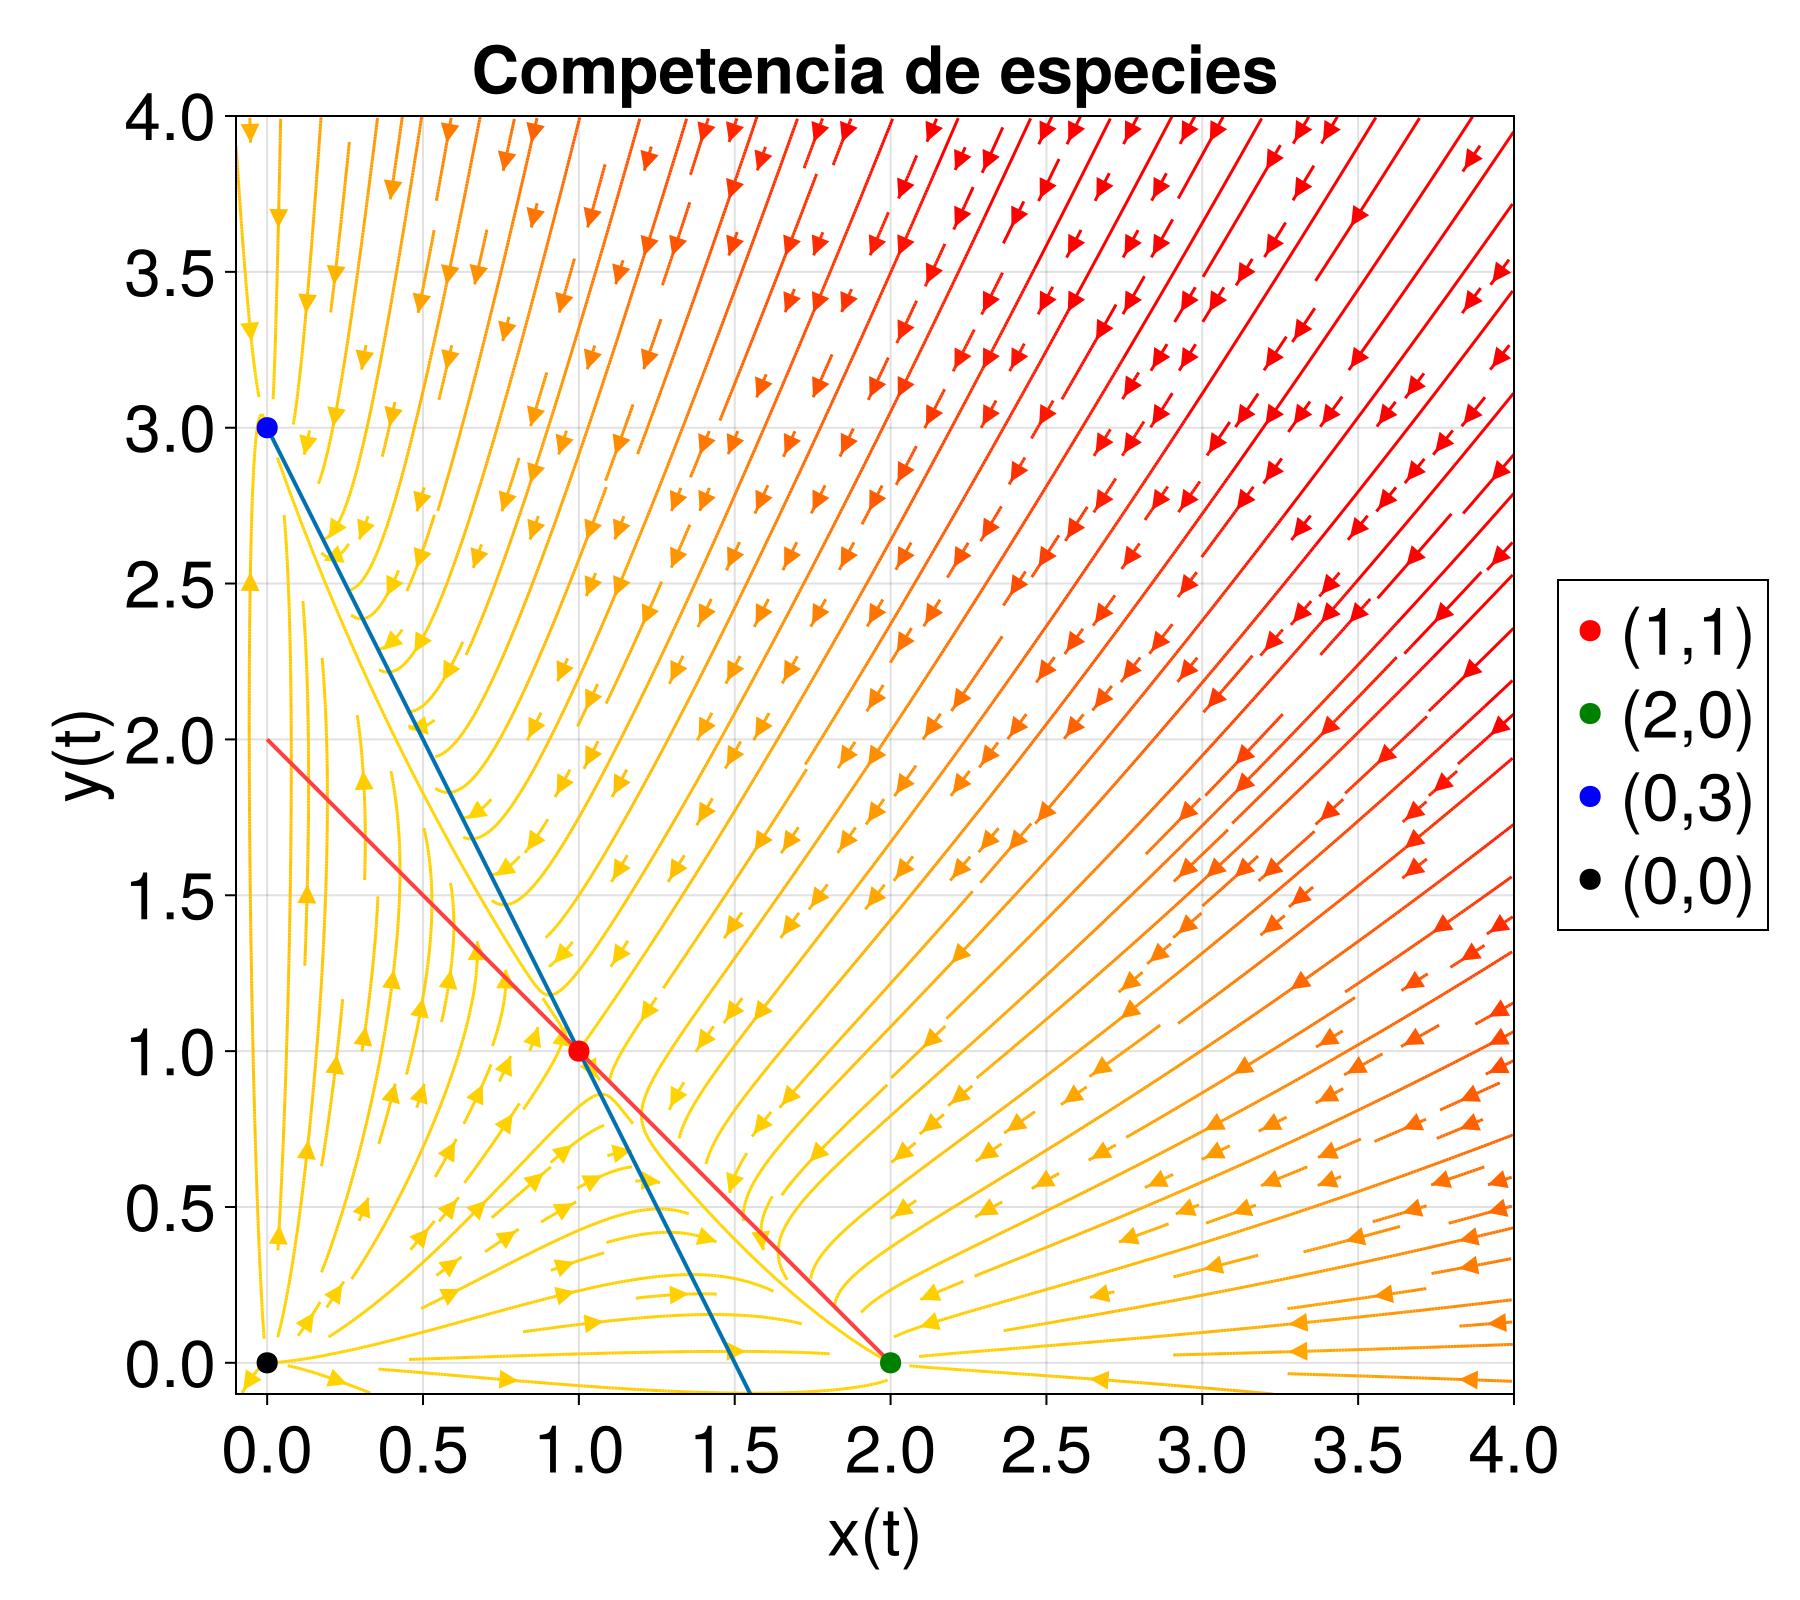
\includegraphics[width=0.5\textwidth]{../Imagenes/Competencia de especies} 
	\end{center} 
	\vspace{-20pt} 
	\caption{Campo vectorial de las soluciones del sistema (\ref{eqn:Sist2x2Comp}) de dos especies.} 
	\vspace{10pt}
	\label{fig:CompetenciaEspecies}
\end{wrapfigure} 
(dependiendo de la dirección y magnitud de la perturbación).
\setlength{\parindent}{0cm} Además de obtener información visual acerca de la estabilidad de los puntos críticos, es posible visualizar las isoclinas del sistema que no son más que el conjunto de puntos donde se satisface:
\begin{equation*}
	\dot{x}=f(x,y)=0,\qquad\dot{y}=g(x,y)=0
\end{equation*}
de modo que en estas rectas una de las dinámicas permanece constante mientras que la otra tiene se mueve hacia arriba o abajo, izquierda o derecha según sea el caso. Como se puede observar, de la representación visual se pueden deducir muchos elementos importantes del sistema, ¿qué pasa cuando el número de ecuaciones no lineales ya no permite la representación visual del espacio fase? Una alternativa sería generar sub-espacios fase que puedan brindar una idea de como es la dinámica a nivel local, pero para ello se tendría que contar con algunos puntos fijos de interés. Sin embargo generar un gran número de gráficas solo para obtener conclusiones puede no ser una buena práctica, para ello existe una técnica analítica de la que ya se ha hablado, que servirá para determinar la estabilidad sin tener que recurrir a una gráfica.
\\
\\
En la sección (\ref{sec:Antecedentes}) se había mencionado que el proceso que llevó a cabo Robert May para poder explorar el sistema a nivel local, consistía en \textit{linealizar} el mismo a través de contar con una función vectorial $\textbf{F}$ no lineal y definir una matriz $A$ tal que sus entradas son $a_{ij}=\left .\frac{\partial f_i(X)}{\partial x_j}\right |_{X^*}$ que es equivalente a definir la matriz Jacobiana de $\textbf{F}$ evaluada en $X^*$.
\newpage
\begin{definición}\label{def:LKVectorial}
	Sea la función vectorial $\mathbf{F}:\mathbb{R}^n\to\mathbb{R}^n$ no lineal y asociada al sistema de Lotka-Volterra de especies en competencia. Se definen sus entradas de la siguiente manera
	\begin{equation}\label{eqn:Fmatricial}
		\mathbf{F}(X)=\begin{pmatrix}
			f_1(X)=r_1x_1\left(1-\frac{\sum_{j=1}^n \alpha_{1j}x_j}{K_1}\right)\\
			\vdots\\
			f_n(X)=r_nx_n\left(1-\frac{\sum_{j=1}^n \alpha_{nj}x_j}{K_n}\right)
		\end{pmatrix},\qquad\text{donde $X(t)=\left(x_1(t),...,x_n(t))\right)\in\mathbb{R}^n$.}
	\end{equation}
	Por lo tanto el sistema (\ref{eqn:LK}) puede ser re-escrito de una forma más compacta considerando
	\begin{equation}\label{eqn:LKmatricial}
		\dot{X}(t) = \mathbf{F}(X(t))
	\end{equation}
	Teniendo ahora la función vectorial que define al sistema de Lotka-Volterra, es directo definir la matriz Jacobiana para poder linealizar el sistema
	\begin{equation}\label{eqn:Jacobiano}
		\mathbb{J}_\mathbf{F}(X^*) = \begin{pmatrix}
			\frac{\partial f_1(X^*)}{\partial x_1} & \cdots &\frac{\partial f_1(X^*)}{\partial x_n}\\
			\vdots & \ddots & \vdots\\
			\frac{\partial f_n(X^*)}{\partial x_1} & \cdots &\frac{\partial f_n(X^*)}{\partial x_n}
		\end{pmatrix}
	\end{equation}
	Se necesitarán puntos fijos de interés y evaluarlos para poder obtener el sistema linealizado.
\end{definición}

\setlength{\parindent}{0cm}Validando esta aseveración, se continúa con el ejemplo \ref{eg:2x2} determinando cada matriz jacobiana y su estabilidad asociada. Se comparará con lo que se muestra en la Figura (\ref{fig:CompetenciaEspecies}). La matriz jacobiana para este sistema es:
\begin{equation}\label{eqn:Jacobiano2}
	\mathbb{J}_\mathbf{F}(X)=\begin{pmatrix}
		r_1-\frac{2r_1\alpha_{11}x_1+r_1\alpha_{12}x_2}{K_1} & -\frac{r_1a_{12}x_1}{K_1}\\
		-\frac{r_2a_{21}x_2}{K_2} & r_2-\frac{2r_2\alpha_{22}x_2+r_2\alpha_{21}x_1}{K_2}
	\end{pmatrix}
\end{equation}
considerando que las entradas $\alpha_{ii}=1$ debido a como se define la matriz de incidencias (\ref{eqn:mIncidencias}). Sustituyendo y operando sobre nuestro sistema, al evaluar los puntos fijos antes encontrados se tienen las siguientes matrices de interacciones:
$$
\mathbb{J}_{(2,0)} = \begin{pmatrix}
	-2 & -2\\
	0 & -1
\end{pmatrix},\qquad \mathbb{J}_{(0,3)}=\begin{pmatrix}
	-1 & 0\\
	-6 & -3
\end{pmatrix},\qquad \mathbb{J}_{(1,1)}=\begin{pmatrix}
	-1 & -1\\
	-2 & -1
\end{pmatrix},\qquad \mathbb{J}_{(0,0)}=\begin{pmatrix}
	2 & 0 \\
	0 & 3
\end{pmatrix}
$$
%%%%%%%%Checkpoint
Teniendo las matrices, solo resta determinar sus valores propios y evaluar sus partes reales para concluir con el tipo de estabilidad asociado a cada uno de los puntos fijos. Realizando el álgebra correspondiente se encuentra lo siguiente
%Por lo tanto los valores propios de las primeras dos matrices de interacciones deben ser negativos para que sustenten los atractores de la figura (\ref{fig:CompetenciaEspecies}). Mientras que los valores propios de $\mathbb{J}_{(1,1)}$ deben ser uno negativo y otro positivo para sustentar al punto silla. Para el caso de la matriz $\mathbb{J}_{(0,0)}$ sus valores propios deben tener parte real positiva para que sustenten el repulsor. 
\begin{align*}
	\mathbb{J}_{(2,0)}&\Longrightarrow\ \lambda_1 = -2,\quad\lambda_2 = -1\\
	\mathbb{J}_{(0,3)}&\Longrightarrow\ \lambda_1 = -3,\quad\lambda_2 = -1\\
	\mathbb{J}_{(1,1)}&\Longrightarrow\ \lambda_1 = -1+\sqrt{2},\quad\lambda_2 = -1-\sqrt{2}\\
	\mathbb{J}_{(0,0)}&\Longrightarrow\ \lambda_1 = 2,\quad\lambda_2 = 3\\
\end{align*}
Se puede observar que las partes reales coinciden con la estabilidad de cada punto fijo de la Figura (\ref{fig:CompetenciaEspecies}). Esta técnica resultará muy útil para cuando se tengan que resolver los sistemas con $N\gg 1$ ecuaciones diferenciales. La parte real de los valores propios de $\mathbb{J}_{\textbf{F}}(X^*)$ determinarán su estabilidad.
%%%%%%%%% Checkpoint
\section{Generalizando a $N\gg 1$ especies.}

Con base en la sección anterior, se tiene una idea de como resolver el sistema dinámico de Lotka-Volterra (\ref{eqn:LK}); en principio se requiere hallar puntos fijos que satisfagan $\textbf{F}(X^*)=\vec{0}$ para poder hallar la matriz Jacobiana del sistema (\ref{eqn:Jacobiano}) y así poder explorar su estabilidad. Todo este proceso se debe de implementar mediante algoritmos los cuales se irán revisando en la sección (apéndice tal\footnote{agregar seccion.}). Sin embargo, en lo que corresponde a esta sección será en definir las interacciones entre especies del sistema mediante la \textit{matriz de incidencias} y ver que parámetros la gobiernan para poder plantear una serie de experimentos/simulaciones que resuelvan las conjeturas planteadas.
\\
\\
Para comenzar el modelado de las interacciones de (\ref{eqn:LK}), es necesario comenzar a hablar de redes/grafos, ya que con este artilugio matemático se podrán representar a las especies de manera conveniente, sobre todo para poder investigar las implicaciones de poder probar con diversas topologías de red por ejemplo: libres de escala, de mundo pequeño o como en nuestro caso: aleatorias. Una red es considerada una colección de \textit{nodos} que se encuentran unidos por \textit{enlaces} \cite{newman2018networks}. Para definir redes siempre es necesario establecer que es lo que representan los nodos y los enlaces, en nuestro caso los nodos representan directamente las especies que participan en el sistema mientras que los enlaces (con pesos) serían sus interacciones.\\
\\
Si se define un conjunto de especies $x_i$ y sabemos que se relacionan por medio de los coeficientes $\alpha_{ij}$ que
\begin{wrapfigure}{l}{0.45 \textwidth} \vspace{-30pt} \begin{center}
		\includesvg[width=.5\textwidth]{../Imagenes/karateLu} 
	\end{center} 
	\vspace{-20pt} 
	\caption{Red de Karate de Zachary} 
	\vspace{-20pt}
	\label{fig:RedKarate}
\end{wrapfigure} 
aparecen en las ecuaciones de (\ref{eqn:LK}), entonces las interacciones entre las especies $x_i$ y $x_j$ se dan para cuando $\alpha_{ij}\neq 0$, y éste representaría el peso del enlace $j\to i$ de la red que se tiene en mente. En el mundo es posible encontrar diferentes tipos de redes con cierto significado, tales como la red de energética de un país, redes de amistades en una universidad o redes de acciones que cotizan en la bolsa de valores; en el caso de la Figura (\ref{fig:RedKarate}) es una red conocida como \href{https://en.wikipedia.org/wiki/Zachary%27s_karate_club}{Red del club Karate de Zachary} \cite{newman2018networks}. Todo tipo de red tiene una representación algebraica que conviene mucho tener en cuenta para la construcción del modelo, es conocida como la \textit{matriz de adyacencia.}\\
\\
\begin{definición}\label{def:matrizdeadyacencia}
	Sea $\mathcal{A}\in\mathrm{M}_n(\mathbb{R}) $. Se define la matriz de adyacencia tal que sus entradas son de la siguiente forma
	$$\mathcal{A}_{ij}= 
	\begin{cases}
		1, \ \text{si $\exists$ un enlace entre el nodo $i$ y el nodo $j$.}\\
		0, \ \text{en otro caso}.
	\end{cases}$$
	De esta forma se puede acceder a la estructura de la red sin necesariamente dibujarla como en la Figura (\ref{fig:RedKarate}), cada renglón de la matriz es un nodo y sus columnas son los nodos disponibles que tiene para conectarse, incluso consigo mismo. Si se le agregan pesos al enlace, entonces $\mathcal{A}_{ij}\in\mathbb{R}$. Al pasar a la siguiente etapa de la construcción de la matriz de incidencias $\Lambda$, estos elementos serán escogidos de una distribución estadística. 
\end{definición}
%%%%%%% Checkpoint
\begin{ejemplo}
	Para poder apreciar la matriz de adyacencia definamos una red de 10 nodos y veamos la matriz de adyacencia que le corresponde. Cada nodo ha sido marcado para poderlo identificar y relacionar con la matriz de adyacencia. Los renglones y columnas de la matriz representan los nodos, siendo el primer renglón el primer nodo, el quinto renglón será el quinto nodo; esto pasa de manera equivalente con las columnas, la cuarta columna corresponde con el cuarto nodo, la octava columna corresponde con el octavo nodo. Por tanto, mediante la matriz de adyacencia sabemos que el primer nodo (renglón 1) esta enlazado con el noveno nodo (columna 9) ya que existe un uno, mientras que el primer renglón y la quinta columna hay un cero lo que indica que no existe un enlace entre estos nodos. 
\end{ejemplo}
\begin{wrapfigure}{r}{0.5 \textwidth} \vspace{-30pt} \begin{center}
		\includesvg[width=0.5\textwidth]{../Imagenes/red10Lu} 
	\end{center} 
	\vspace{-20pt} 
	\caption{Red no dirigida de 10 nodos.} 
	\vspace{-150pt}
	\label{fig:Red10}
\end{wrapfigure} 

$$
A=\begin{pmatrix}
	0 & 1 & 0 & 1 & 0 & 0 & 0 & 0 & 1 & 0 \\
	1 & 0 & 1 & 0 & 0 & 1 & 0 & 0 & 0 & 0 \\
	0 & 1 & 0 & 0 & 0 & 0 & 1 & 1 & 0 & 0 \\
	1 & 0 & 0 & 0 & 1 & 1 & 1 & 0 & 0 & 1 \\
	0 & 0 & 0 & 1 & 0 & 0 & 0 & 0 & 1 & 1 \\
	0 & 1 & 0 & 1 & 0 & 0 & 1 & 1 & 0 & 1 \\
	0 & 0 & 1 & 1 & 0 & 1 & 0 & 0 & 1 & 0 \\
	0 & 0 & 1 & 0 & 0 & 1 & 0 & 0 & 1 & 0 \\
	1 & 0 & 0 & 0 & 1 & 0 & 1 & 1 & 0 & 1 \\
	0 & 0 & 0 & 1 & 1 & 1 & 0 & 0 & 1 & 0 \\
\end{pmatrix}
$$\\
\\
También hay que destacar qué la matriz es simétrica y que la diagonal es igual a cero: para el primer punto se debe notar que la relación de los enlaces entre nodos no tiene dirección, es decir, que exista un enlace entre nodos significa que el nodo $i$ se conecta con $j$ y viceversa. Por tanto la red de la figura (\ref{fig:Red10}) es \textit{no dirigida} puesto que no hay una dirección preferencial en el enlace. Para el segundo punto se puede deducir que los nodos podrían relacionarse consigo mismo, en este caso particular no lo hacen pero si es posible la existencia de \textit{autoenlaces}. Para el sistema (\ref{eqn:LK}) estos autoenlaces representan las auto-interacciones que dan el carácter logístico (\ref{eqn:EqLogistica}) de las ecuaciones. Más adelante se hablará de la importancia de estos autoenlaces.
\\
\\
Cuando se tiene el caso en que los enlaces tienen una dirección preferencial de nodo a nodo, se dice que corresponde a una \textit{red dirigida}. En este caso el enlace podrá ir del nodo $i$ al nodo $j$ pero no necesariamente lo hará en sentido contrario, deberá definirse explícitamente. En el mundo también existe un gran conjunto de redes dirigidas como lo son las citaciones académicas, la propia WWW (World Wide Web), incluso redes tróficas. Y para este caso también se tiene asociada una matriz de adyacencia con una ligera modificación con respecto de la definición \ref{def:matrizdeadyacencia}.
\begin{definición}
	Sea $\mathcal{D}\in\mathrm{M}_n(\mathbb{R})$, matriz de adyacencia de una red dirigida. Se definen sus elementos de la siguiente manera:
	$$
	\mathcal{D}_{ij}=\begin{cases}
		1,\qquad\text{Si existe un enlace del nodo $i$ al nodo $j$}\\
		0,\qquad\text{otro caso.}
	\end{cases}
	$$
	Los enlaces de las redes dirigidas van a estar representados por flechas para que puedan mostrar adecuadamente las direcciones correspondientes entre los nodos. Las redes ecológicas que Robert May definió en su trabajo son consideradas dirigidas, ya que el sentido de sus enlace tienen una dirección preferencial.
\end{definición}

\begin{ejemplo}
	Se tiene la siguiente red dirigida de 10 nodos con exactamente 14 enlaces. La matriz de adyacencia asociada es la siguiente
\end{ejemplo}
\begin{wrapfigure}{l}{0.5 \textwidth} \vspace{-44pt} \begin{center}
		\includesvg[width=0.52\textwidth]{../Imagenes/Red10DirLu} 
	\end{center} 
	\vspace{-20pt} 
	\caption{Red dirigida de 10 nodos.} 
	\vspace{-200pt}
	\label{fig:Red10Dir}
\end{wrapfigure} 
$$
D = \begin{pmatrix}
	0 & 0 & 0 & 0 & 0 & 0 & 0 & 0 & 0 & 1 \\
	1 & 0 & 1 & 0 & 0 & 0 & 0 & 1 & 0 & 0 \\
	0 & 0 & 0 & 1 & 1 & 0 & 0 & 0 & 0 & 1 \\
	1 & 0 & 0 & 0 & 0 & 0 & 0 & 0 & 0 & 0 \\
	0 & 0 & 1 & 0 & 0 & 0 & 0 & 1 & 0 & 0 \\
	0 & 1 & 0 & 0 & 0 & 0 & 0 & 0 & 0 & 0 \\
	0 & 0 & 1 & 0 & 0 & 0 & 0 & 0 & 0 & 0 \\
	0 & 0 & 0 & 0 & 0 & 0 & 0 & 0 & 0 & 0 \\
	0 & 1 & 0 & 0 & 0 & 0 & 0 & 0 & 0 & 0 \\
	0 & 0 & 0 & 0 & 0 & 0 & 1 & 0 & 0 & 0 \\
\end{pmatrix}
$$
\newpage
Ahora se puede notar que la matriz de adyacencia no es simétrica y que en consecuencia los enlaces presentan una dirección preferencial. Ambas visiones se van a tomar en cuenta para modelar al sistema (\ref{eqn:LK}) generalizado, sin embargo, tendrá mayor protagonismo la \textit{red no dirigida} sobre la otra, ya que en un principio los experimentos fueron diseñados bajo esta lógica. Habiendo definido las redes y sus matrices de adyacencia, se debe seguir el camino definiendo que tipo de red se ocupará para el modelo.

\subsection{Red de incidencias}

La \textit{red de incidencias} será la representación de la relación entre especies bajo la lógica del sistema de Lotka-Volterra generalizado; dicha red tiene asociada su matriz de adyacencia que se denominará \textit{matriz de incidencias} la cual tendrá tres principales características: puede ser de una red dirigida o no dirigida, definir la dirección de las interacciones hace más completo al sistema, sin embargo se usarán mayormente redes no dirigidas. La topología de la red que se va a utilizar es la de Erdös–Rényi \cite{posfai2016network} conocida por tener un carácter aleatorio con base en una probabilidad $p$. Y aunado a todo ello se considerará un peso para cada enlace cuyo valor vendrá de una distribución normal centrada en $\mu=0$ y desviación estándar $\sigma$.\\
\\
La red de Erdös–Rényi es ampliamente utilizada para aprender sobre la estructura y propiedades de la redes y con ello poder extender ese aprendizaje al estudio de las llamadas \textit{redes libres de escala}. La diferencia sustancial entre la red aleatoria y la red libre de escala es que la primera tiene muy pocas (o ninguna) aplicaciones en escenarios de la naturaleza \cite{posfai2016network}. Las estructuras en la naturaleza están representadas matemáticamente por las redes libres de escala, siguiendo leyes de potencia y otra variedad de propiedades. Sin embargo este trabajo únicamente se centrará en el uso del modelo de Erdös–Rényi aplicado al sistema (\ref{eqn:LK}) para tener un primer acercamiento a la dinámica que produce, con intenciones de extender el estudio al caso de las redes libres de escala\footnote{Un modelo teórico que rescata todas las propiedades de las redes libres de escala es el de Albert-Barabasi \cite{posfai2016network}.}. 
\begin{definición}\label{def:redAleatoria}
	Sea un conjunto de $N$ nodos sin enlaces asociados. Se define la red aleatoria $\mathcal{G}_\mathcal{E}$ con su matriz de adyacencia asociada $\mathcal{E}\in\mathrm{M}_n(\mathbb{R})$ si para cada par de nodos $n_i$ y $n_j$ de las $\binom{N}{2}$ posibles combinaciones se definen sus enlaces aleatorios dada una probabilidad $p$ y un número aleatorio $r\in[0,1]$ con base en la siguiente regla:
	$$
	L_{ij}=\begin{cases}
		\exists,\qquad\text{Si }r<p\\
		\nexists,\qquad\text{Si }r\geq p
	\end{cases},\qquad L_{ii}=0
	$$
	desde luego que entre mayor sea la $p$ se tendrá mayor cantidad de enlaces. En este caso no se anuncia una dirección preferencial, por lo que la red aleatoria de Erdös–Rényi es \textit{no dirigida}\footnote{En esta referencia \cite{posfai2016network} el lector podrá conocer más sobre sus propiedades.}. Ya que $\mathcal{G}_\mathcal{E}$ es no dirigida, su matriz de adyacencia $\mathcal{E}$ es simétrica. \\
	\\
	Sin embargo, es posible extender esta definición a redes aleatorias dirigidas suponiendo que la conexión tiene dirección preferencial, por lo tanto ahora existirán $N(N-1)$ posibles combinaciones de nodos. Si solo se considerara uno de los dos casos, es decir, para $\binom{N}{2}$ combinaciones de nodos entonces se tendría la mitad de posibles conexiones, la matriz de adyacencia sería triangular superior por haber considerado únicamente la dirección de $n_i$ a $n_j$. Para llenar la parte triangular inferior de esta matriz se deben considerar las conexiones de $n_j$ a $n_i$, como resultado ahora se tiene una red aleatoria dirigida cuya matriz de adyacencia es no simétrica. En la sección (\ref{sec:RedesAleatorias}) se encuentra la implementación computacional de ambas visiones de la red aleatoria.
\end{definición}
\setlength{\parindent}{0cm}En este punto solamente falta de considerar la magnitud de las interacciones entre especies para terminar de construir la matriz de incidencias. Para ello se va a tomar en cuenta una matriz de $\mathcal{M}\in\mathrm{M}_n(\mathbb{R})$ que estará mapeada con valores que vienen de una distribución normal centrada en $\mu=0$ y desviación estándar $\sigma$, es decir, $\mathcal{M}_{ij}\in\mathcal{N}(0,\sigma)$.
\begin{definición}\label{def:MatrizIncidencias}
	Sea una red aleatoria $\mathcal{G}_\mathcal{E}$ dirigida o no dirigida con matriz de adyacencia $\mathcal{E}\in\mathrm{M}_n(\mathbb{R})$. Sea una matriz $\mathcal{M}\in\mathrm{M}_n(\mathbb{R})$ de entradas aleatorias provenientes de una distribución normal $\mathcal{N}(0,\sigma)$. Se define a $\Lambda$ la \textit{matriz de incidencias} como el producto de Hadamard \cite{HadamardProduct} de la matriz de adyacencia con la matriz de entradas aleatorias sumada con la matriz identidad:
	\begin{equation}\label{eqn:MatrizIncidencias}
		\Lambda=(\mathcal{E}\odot \mathcal{M}) + I
	\end{equation}
	El producto agrega pesos de la distribución normal a cada posible enlace de la red aleatoria y la suma con de la identidad es para poder agregar autoenlaces de peso $1$ a cada nodo de la misma.
\end{definición}
\setlength{\parindent}{0cm} La matriz de incidencias $\Lambda$ puede ser \textit{estructuralmente simétrica}\footnote{Es una matriz cuyas entradas cumplen $B_{ij}\neq B_{ji}\neq 0$ ó $B_{ij}=B_{ji}=0$ para toda $B_{ij}\in B$, quiere decir que aunque $B$ no sea simétrica, relativo a las posiciones de sus entradas si lo es.} si se escoge una red $\mathcal{G}_\mathcal{E}$ no dirigida, o puramente aleatoria si se escoge la opción  de red dirigida. Las implicaciones más importantes de esta distinción es que para $\Lambda$ estructuralmente simétrica únicamente podrán existir 3 tipos de interacciones mientras que la puramente aleatoria considera hasta 5 de ellas posibles. Los elementos $\alpha_{ij}\in\Lambda$ serán los coeficientes de interacción que aparecen en las ecuaciones de (\ref{eqn:LK}) y en este punto se ha concluido un paso más de la construcción del modelo.\\
\\
En la figura (\ref{fig:RedIncidencias}) se muestra una representación visual de las interacciones entre especies de los sistemas por resolver (\ref{eqn:LK}). En la sección (\ref{sec:redIncidencias}) se muestra la implementación computacional de la red de incidencias. En la siguiente sección se hablará acerca de los tipos de interacciones posibles que se pueden tener, para cada caso descrito anteriormente.
\newpage
\begin{wrapfigure}{r}{0.5 \textwidth} \vspace{-70pt} \begin{center}
		\includesvg[width=0.52\textwidth]{../Imagenes/RedIncidencias} 
	\end{center} 
	\vspace{-52pt} 
	\caption{Red de incidencias de 8 nodos bajo la topología de una red aleatoria dirigida con $p=0.15$ y una matriz aleatoria con $\mu=0$ y $\sigma=0.2$.} 
	\vspace{-10pt}
	\label{fig:RedIncidencias}
\end{wrapfigure} 


\subsection{Tipos de interacciones}

La red de incidencias es de tipo dirigida independientemente del tipo de red aleatoria que se decida elegir para su construcción, a lo mucho podrá ser estructuralmente simétrica pero los pesos de cada enlace $i\to j$ y $j\to i$ son diferentes lo que implica que $\alpha_{ij}\neq\alpha_{ji}$ para toda $\alpha_{ij}\in\Lambda$. Puede considerarse como un efecto natural puesto que el nivel de interacción entre especies difícilmente va a ser igual. Existen más interacciones además de la competencia que generan dinámicas interesantes, en esta sección se explorarán dichas interacciones y su aplicación en la matriz de incidencias.
\\
\\
Hasta ahora únicamente se han discutido las ecuaciones de (\ref{eqn:LK}) bajo el escenario de la competencia, es decir para toda $\alpha_{ij}\in\Lambda$ positiva. El caso particular $N=2$ ha develado que este sistema es incapaz de superar sus capacidades de carga, por lo que tienen un crecimiento controlado. Pero ¿qué pasa si se comienzan a considerar $\alpha_{ij}<0$ provenientes de la distribución normal? ¿Cómo podría afectar en la dinámica resultante y qué pasaría con las capacidades de carga del sistema? Para comenzar a explorar las respuestas a estas preguntas hay que definir el tipo de interacciones posibles en $\Lambda$ y May presenta un abanico de 5 de ellas \cite{may2019stability}.\\
\\
Las interacciones a las que May refiere, únicamente se aplican a su \textit{community matrix} que sería lo equivalente a las matrices Jacobianas de nuestro sistema evaluadas en algún punto fijo (\ref{eqn:Jacobiano}). Estas interacciones no necesariamente aplican a la matriz de incidencias $\Lambda$, sin embargo podrán aplicarse  si se les voltean el signo tal y como se verá más adelante. Las posibles interacciones se reparten de la siguiente forma: para sistemas de May con matrices estructuralmente simétricas únicamente podrán acceder a tres tipos de interacción, las de competencia $(--)$, las de cooperación\footnote{Conocidas también por mutualismo o simbiosis.} $(++)$ y las de presa-depreador $(+-)$ ó $(-+)$.
\\
\\
Cuando se tienen sistemas de May puramente aleatorios entonces pueden acceder a los 5 tipos de interacción, ya que su matriz de interacciones puede contener entradas estructuralmente simétricas aunque en general no lo sea. Las interacciones que faltan son: el comensalismo $(+0)$, amensalismo $(-0)$. \\
\\
La relación de cooperación implica que ambas especies se verán beneficiadas de su interacción mutua, en contraste con la competencia en la que ambas se van a ver perjudicadas. Para el caso de la interacción presa-depredador, una de las especies se verá beneficiada mientras que la otra saldrá perjudicada de dicho beneficio. En el  comensalismo una de las especies se beneficia mientras que la otra no presenta ningún impacto. Por el contrario, en el amensalismo una de las especies se perjudica mientras que la otra no presenta algún cambio.

\subsubsection*{Interacciones de May aplicadas a la red de incidencias}

Las interacciones que se aplican a la matriz de incidencias son las mismas que May estipula para sus matrices de interacción solamente que con el signo contrario. Para el caso de la competencia se tendrán $(++)$, en cooperación serán $(--)$, presa-depredación $(-+)$ ó $(+-)$, comensalismo $(-0)$ y por último amensalismo $(+0)$. Para poder ver de que forma afectan los coeficientes $\alpha_{ij}\in\Lambda$ provenientes de la distribución normal $\mathcal{N}(0,\sigma)$, extendemos las ecuaciones del sistema (\ref{eqn:LK}) de modo que
\begin{equation}\label{eqn:LKextendida}
	r_ix_i\left (1 - \frac{\alpha_{ii}x_i+\alpha_{i1}x_1+\cdots+\alpha_{iN}x_N}{K_i}\right )\quad\Longleftrightarrow\quad r_ix_i\left (1-\frac{\alpha_{ii}x_i}{K_i}\right )-r_ix_i\left (\frac{\sum_{j\neq i}\alpha_{ij}x_j}{K_i}\right )
\end{equation}
El sistema se puede separar en una componente logística y en una suma de términos no lineales. Para que la componente logística mantenga regulado su crecimiento (omitiendo el resto de términos), es necesario que $\alpha_{ii}>0$, por simplicidad y convenciencia se ha definido en la matriz de incidencias que todos estos elementos sean $\alpha_{ii}=1$, pero en esencia es suficiente con que sean mayor a cero. Observe que si $\alpha_{ii}\leq 0$, entonces el crecimiento será exponencial y sin límites.
\\
\\
Los términos de la suma de (\ref{eqn:LKextendida}) van a aportar valor al término logístico y va a depender del resto de coeficientes $\alpha_{ij}$ junto con su signo. Si el signo es negativo, con el signo menos de la izquierda se hará positivo y entonces agregará crecimiento a la dinámica de $x_i$, este escenario puede suceder en interacciones de cooperación, en la interacción depredador únicamente y en el comensalismo. Por el contrario si $\alpha_{ij}>0$ entonces va a restar crecimiento a la dinámica de $x_i$ (tal y como se aprecia en el ejemplo \ref{eg:2x2}). En contraparte, este escenario se va a dar en la competencia, en la presa únicamente y en el amensalismo. Nótese que cuando $\alpha_{ij}=0$ no incurre en algún cambio en $x_i$. \\
\\
Las interacciones negativas que agregan valor al crecimiento de cada especie, generan la oportunidad de que dicho incremento logre sobrepasar la(s) capacidad(es) de carga del sistema, lo que puede generar que el punto de estabilidad de las especies quede por arriba de dichas $K_i$, algo que no se permite en el sistema puramente de competencia. Sin embargo, debe de existir un balance entre las interacciones positivas y negativas, ya que si las segundas se sobreponen a las primeras, puede ocurrir un colapso del sistema traducido en crecimiento desmedido. Este escenario corresponderá a aquellos sistemas (\ref{eqn:LK}) inestables resultantes de ciertas configuraciones en $p$, $\sigma$ y $N$ de la matriz de incidencias y se irá revisando más adelante.\\
\\
Dependiendo de la $p$ que forma la matriz de incidencias, cada especie podrá tener a lo mucho $N$ interacciones posibles con fuerza promedio $\sigma$, lo que implica que cada especie puede tener interacciones de cooperación, competencia, etc, de forma aleatoria (dependiendo si la matriz es estructuralmente simétrica o no). La dinámica resultante se acompleja conforme $N$ es mayor debido a todo el cúmulo de posibles interacciones en la que cada una de ellas afecta significativamente al desarrollo de cada especie. Partiendo de la estructura aleatoria de la red y el peso de las interacciones provenientes de $\mathcal{N}(0,\sigma)$, es complejo de idear tan si quiera un bosquejo de la dinámica resultante del sistema (\ref{eqn:LK}).

\subsubsection*{Interacciones de $\Lambda$ para $N=2$.}

\begin{ejemplo}\label{eg:2x2CoopyDemás}
	Se explorará un caso particular de un sistema (\ref{eqn:LK}) para $N=2$ con interacciones de cooperación. Se corroborará si efectivamente su dinámica es capaz de sobrepasar sus capacidades de carga. A través del espacio fase y las series de tiempo se observará dicho fenómeno. El sistema en concreto es
	\begin{equation}\label{eqn:Sist2x2Coop}
		\begin{split}
			\frac{dx}{dt} &= 2x\left (1-\frac{x}{2}\right )+\frac{1}{2}xy\\
			\frac{dy}{dt} &= 3y\left (1-\frac{y}{3}\right )+xy
		\end{split}
	\end{equation}
	La matriz de incidencias asociada a este caso sería 
	$$
	\Lambda = \begin{pmatrix}
		1 & -\frac{1}{2}\\
		-1 & 1
	\end{pmatrix}
	$$
	A diferencia del sistema del Ejemplo \ref{eg:2x2} (Ec. \ref{eqn:Sist2x2Comp}) su anti-diagonal es negativa lo que indica que son coeficientes de interacción $(--)$ que propician la cooperación entre especies y fomentan sus crecimientos. Los puntos fijos para este sistema ahora son: $(0,0)$, $(2,0)$, $(0,3)$ y $(7,10)$; las matrices jacobianas asociadas son:
	$$
	\mathbb{J}_{(0,0)}=\begin{pmatrix}
		2 & 0 \\
		0 & 3
	\end{pmatrix},\qquad\mathbb{J}_{(2,0)}=\begin{pmatrix}
	-2 & 1\\
	0 & 5
	\end{pmatrix},\qquad\mathbb{J}_{(0,3)}=\begin{pmatrix}
	3.5 & 0 \\
	3 & -3
	\end{pmatrix},\qquad\mathbb{J}_{(7,10)}=\begin{pmatrix}
	-7 & 3.5\\
	10 & -10
	\end{pmatrix}
	$$
	Realizando el cálculo de los valores propios de cada una de las matrices de interacción se encuentra que para el primer punto fijo se tiene el conocido y trivial repulsor. En el caso de los puntos fijos de los ejes ahora su estabilidad ha cambiado con respecto del sistema (\ref{eqn:Sist2x2Comp}), se tienen puntos sillas que resultan ser inestables ya que para $t\to\infty$ las soluciones terminan divergiendo. Por último se encuentra que los valores propios del punto fijo restante son negativos, lo que implica que todas las soluciones del sistema irán a converger a este punto.
	\begin{figure}[h!]
		\centering
		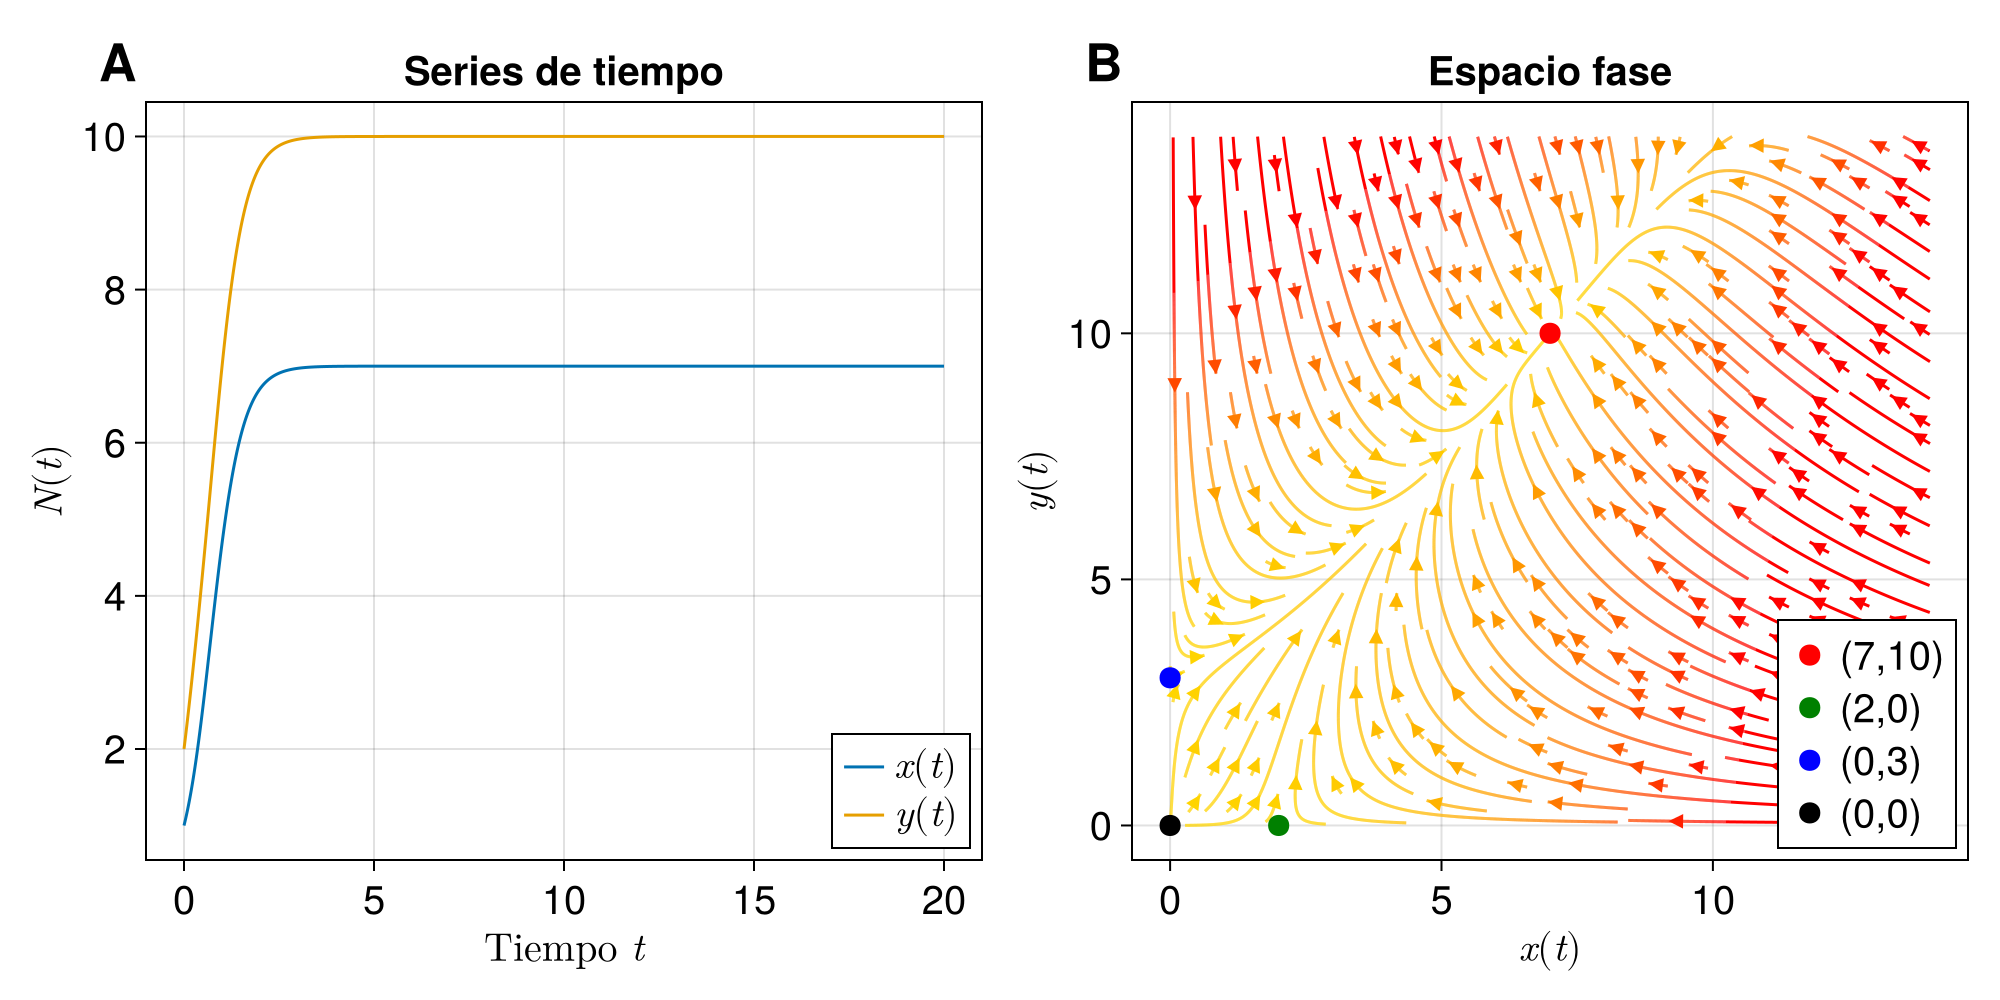
\includegraphics[scale=0.24]{../Imagenes/Cooperacion de especies}
		\caption{Sistema de Lotka-Volterra con interacciones de cooperación dados por las ecuaciones (\ref{eqn:Sist2x2Coop}). Tasas de crecimiento y capacidades de carga: $r_x=K_x=2$ y $r_y=K_y=3$. \textbf{A}) Series de tiempo del sistema para las especies $x(t)$ y $y(t)$ bajo la condición inicial $(1,2)$. (\textbf{B}) Espacio fase del sistema con sus puntos fijos asociados, se muestra solamente un único punto fijo estable.}
		\label{fig:CooperacionEspecies}
	\end{figure}\\
	\\
	 Esto es cuanto menos interesante, ya que se puede observar que efectivamente la cooperación entre las especies $x$ y $y$ es capaz de superar sus propias capacidades de carga que fungían como límites. Bajo este escenario el concepto de la capacidad de carga podría tomar otro significado: ahora será un parámetro que regule el crecimiento de las especies, cuanto mayor sea la capacidad de carga será más difícil el crecimiento de las $x_i$; en caso contrario podrá haber una fácil apertura para el crecimiento desmedido debido a que las $K_i$ no serán capaces de contener las interacciones $\alpha_{ij}<0$. Aunque por su puesto también va dependerá de la magnitud de las $\alpha_{ij}\in\Lambda$.\\
	 \\
 	La cooperación entre especies fomenta su crecimiento y ahora su estabilidad se posiciona en puntos que quedan por arriba de sus capacidades de carga. Cuando se tienen las interacciones comensalismo (-0) y amensalismo (+0), solo una de las especies seguirá su comportamiento logístico mientras que la otra encontrará su estabilidad arriba o debajo de su capacidad de carga. La interacción de depredación $(-+)$ la especie depredadora se estabiliza arriba de su $K_i$ y la presa por debajo de la misma.\\
 	\\
 	Se modifica el sistema (\ref{eqn:Sist2x2Coop}) de tal modo que se considere cada una de estas interacciones. En este caso se elige que $\alpha_{21}=0$ de la ecuación $\dot{y}$ y $\alpha_{12}=\pm\frac{1}{2}$ de la ecuación $\dot{x}$ para cubrir los casos de comensalismo y amensalismo. La ecuación $\dot{y}$ queda reducida a una ecuación logística, la cual no se verá afectada por la dinámica de $\dot{x}$ y se mantendrá estable en su capacidad de carga. \\
 	\\
 	\begin{figure}[h!]
 		\centering
 		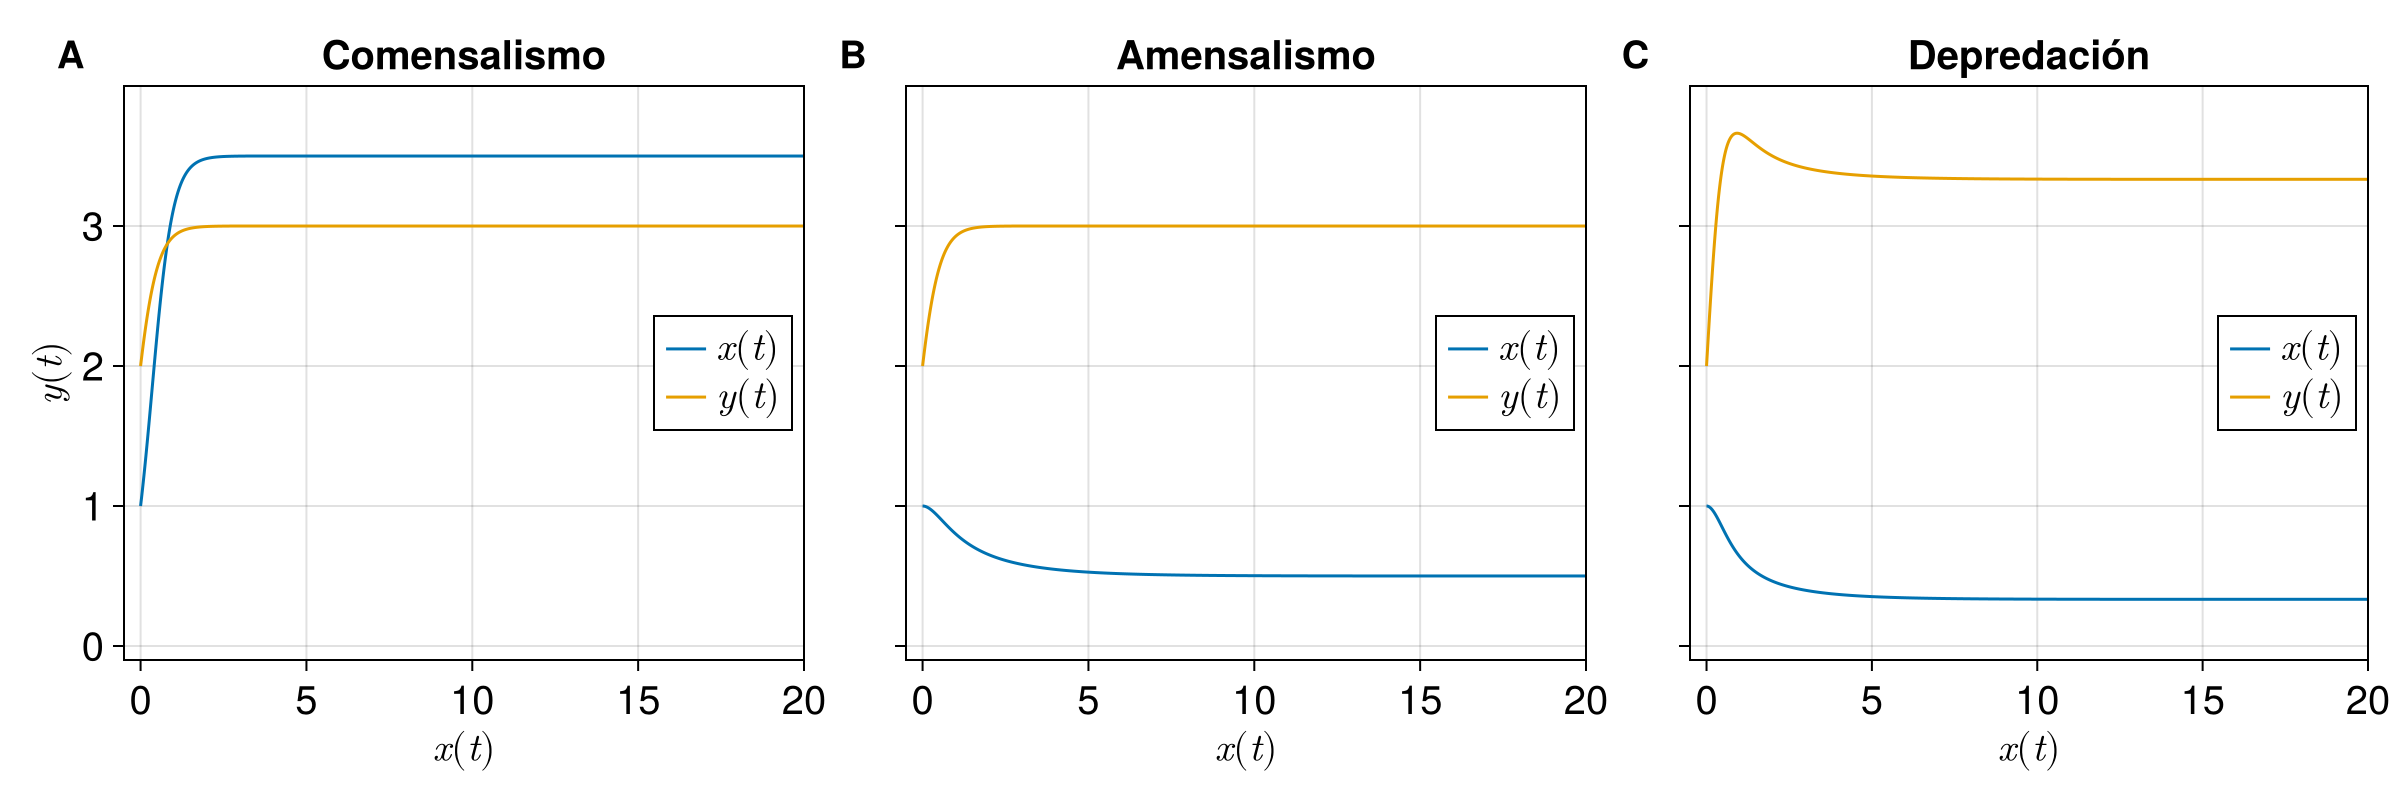
\includegraphics[scale=0.2]{../Imagenes/STrestoInteracciones}
 		\caption{Series de tiempo para las interacciones comensalismo, amensalismo y depredación. (\textbf{A}) Para el comensalismo se definió $\alpha_{21}=0$ y $\alpha_{12}=-\frac{1}{2}$. (\textbf{B}) Para el amensalismo se consideró $\alpha_{21}=0$ y $\alpha_{12}=\frac{1}{2}$ (\textbf{C}) Para la depredación se consideró $\alpha_{21}=-1$ y $\alpha_{12}=\frac{1}{2}$.}
 		\label{fig:RestoInteraccionesST}
 	\end{figure}
 	
	Para el caso de depredación se utiliza $\alpha_{12}=\frac{1}{2}$ y $\alpha_{21}=-1$ y es como una combinación de los anteriores, una de las especies logra estabilizarse en un punto superior a su capacidad de carga mientras que la otra se establece en algún punto menor a su capacidad de carga pero sin llegar a extinguirse. En estos casos particulares los coeficientes $\alpha_{ij}<0$ fueron soportados sus capacidades de carga, pero dependiendo de su magnitud es que pudo desenvolver en sistemas estables. Hasta el momento, la estabilidad va a depender de: la magnitud de las capacidades de carga y los coeficientes de interacción en relación a las anteriores.
\end{ejemplo}
En esta sección se ha construido la matriz de incidencias $\Lambda$ necesaria para definir las interacciones del sistema (\ref{eqn:LK}). Se hizo con base en una red de Erdös–Rényi dirigida o no dirigida, contemplando que el peso de los enlaces provienen de una distribución normal centrada en cero y desviación estándar $\sigma$, y agregando autoenlaces con peso $1$. Posteriormente se revisaron las posibles interacciones que se pueden obtener de $\Lambda$ siendo 3 o hasta 5 dependiendo del tipo de red aleatoria escogida. Se ha analizado que los coeficientes $\alpha_{ii}$ deben ser positivos para que respeten el comportamiento logístico de cada especie, y que los coeficientes $\alpha_{ij}<0$ son capaces de agregar valor al crecimiento de las especies hasta sobrepasar sus capacidades de carga. Por último se ha explorado que la estabilidad va a depender del balance entre coeficientes positivos y negativos en conjunción con las capacidades de carga en términos de sus magnitudes.
\\
\\
Por lo tanto ya se tiene todo para comenzar a integrar numéricamente el sistema para cualquier $N$, el siguiente paso será determinar la matriz Jacobiana del sistema para analizar aspectos alrededor de ella. En la sección (\ref{sec:poblacionesLK}) se muestra la implementación computacional de este sistema.

\section{Jacobiana del sistema}

Anteriormente se ha comentado sobre la \textit{linealización} del sistema para conocer la estabilidad alrededor de un punto fijo. Se ha definido la forma vectorial del sistema de Lotka-Volterra generalizado (\ref{eqn:LKmatricial}) y se definió su matriz \textit{Jacobiana} (\ref{eqn:Jacobiano}) en su representación general. En esta sección se va a definir la forma explícita de esta matriz Jacobiana para cualquier número de especies, y se corroborará si las interacciones resultantes se ajustan con las May definió en \cite{may2019stability}. Con esto se abrirá paso a hablar sobre la estabilidad de este sistema en términos de los parámetros que gobiernan a $\Lambda$.\\
\\
Con base en la definición \ref{def:LKVectorial} se define el sistema de Lotka-Volterra generalizado como $\dot{X}=\textbf{F}(X)$, siendo \textbf{F} la función vectorial no lineal del sistema. Para determinar su matriz Jacobiana se tienen que aplicar las derivadas parciales a cada $f_i(X)\in\mathbf{F}(X)$ y para ello separamos en dos casos: considerando elementos de la diagonal $\frac{\partial f_i(X)}{\partial x_i}$, y para aquellos que quedan fuera de la diagonal: $\frac{\partial f_i(X)}{\partial x_k}$; tomamos las ecuaciones del sistema (\ref{eqn:LK}) para realizar el cálculo:
$$
f_i(X) = r_ix_i\left (1-\frac{\sum_{j=1}^N \alpha_{ij}x_j}{K_i}\right )
$$
para los términos de la diagonal se tiene
\begin{equation}\label{eqn:Jacobiano_ii}
	\begin{split}
			f_i(X) &= r_ix_i - \frac{\sum_{j=1}^N r_i\alpha_{ij}x_ix_j}{K_i} \\
			\frac{\partial f_i(X)}{\partial x_i} &= r_i -
			\frac{2r_i\alpha_{ii}x_i+\sum_{j\neq i} r_i\alpha_{ij}x_j}{K_i}\\
			\frac{\partial f_i(X)}{\partial x_i} &= r_i \left (1-\frac{2\alpha_{ii}x_i+\sum_{j\neq i}\alpha_{ij}x_j}{K_i}\right )
	\end{split}
\end{equation}
y para los términos que quedan fuera de la diagonal tenemos
\begin{equation}\label{eqn:Jacobiano_ij}
		\frac{\partial f_i(\vec{x})}{\partial x_k} = -\frac{r_i\alpha_{ik}x_i}{K_i} 
\end{equation}
\begin{definición}\label{def:MatrizJacobiana}
	Sea $\mathcal{J}\in\mathrm{M}_N(\mathbb{R})$ donde $N$ es el número de especies del sistema de Lotka-Volterra generalizado. Se define la matriz \textit{Jacobiana} asociada al sistema (\ref{eqn:Fmatricial}) de la siguiente forma
	\begin{equation}\label{eqn:MartizJacobiana}
		\mathcal{J}=\begin{cases}
			\mathcal{J}_{ii} = r_i \left (1-\frac{2\alpha_{ii}x_i+\sum_{k\neq i}\alpha_{ik}x_k}{K_i}\right ),\qquad&\text{para }i\in\{1,...,N\}\\
			\mathcal{J}_{ij} = -\frac{r_i\alpha_{ij}x_i}{K_i},\qquad&\text{para }i\neq j
		\end{cases}
	\end{equation}
\end{definición}
Teniendo el punto fijo de interés del sistema y evaluándolo en $\mathcal{J}$ se podrá conocer su estabilidad a través del cálculo de sus valores propios. Se puede notar que los elementos fuera de la diagonal de $\mathcal{J}$ voltean el signo con respecto de $\Lambda$, lo que parece ajustarse con las interacciones que May define en su \textit{community matrix} \cite{may2019stability}. Además de voltear el signo, la operación sugiere un re-escalamiento del elemento $\alpha_{ij}$ por lo que en esencia, ¡la matriz Jacobiana es un re-escalamiento de la matriz de incidencias! ¿Qué ocurre con los elementos de la diagonal?
\begin{proposición}\label{prop:DiagonalI}
	Los elementos de la diagonal de la matriz Jacobiana son negativos cuando se evalúa en un punto fijo estable.
	$$
	r_i \left (1-\frac{2x_i+\sum_{j\neq i}\alpha_{ij}x_j}{K_i}\right )<0
	$$	
	\begin{proof}
		Sea $X^*$ un punto fijo estable. Se sabe que la tasa de crecimiento $r_i$ siempre es positiva por lo que la descartamos del análisis. Por otro lado las entradas de $X^*$ son positivas y existen algunas $x_i\in X^*$ tal que son mayores a su capacidad de carga, es decir, $x_i>K_i$ a causa a las $\alpha_{ij}<0$ de la matriz de incidencias. Teniendo en cuenta la siguiente suma
		\begin{equation}\label{proof1:sumaClave}
			2x_i+\sum_{j\neq i}\alpha_{ij}x_j
		\end{equation}
		no se puede asegurar que sea mayor a cero, pues existen tantas $\alpha_{ij}$ negativas como positivas. Suponiendo que son mayores que cero implica que
		$$K_i<2x_i+\sum_{j\neq i}\alpha_{ij}x_j\qquad\Longleftrightarrow\qquad 1-\frac{2x_i+\sum_{j\neq i}\alpha_{ij}x_j}{K_i}<0$$
		Y por lo tanto el elemento $\mathcal{J}_{ii}$ es menor que cero. ¿Qué pasaría si $K_i>2x_i+\sum_{j\neq i}\alpha_{ij}x_j$? La suma (\ref{proof1:sumaClave}) puede ser negativa o positiva pero estrictamente menor a $K_i$ lo que implicaría que el elemento del paréntesis de $\mathcal{J}_{ii}$ sería positivo. Si la matriz Jacobiana tiene elementos de la diagonal positivos entonces se puede asegurar que el sistema será inestable en su punto fijo asociado. Para demostrar esto se recurrirá al \textit{Teorema de Gershgorin} \cite{GershgorinTheorem}. Se asume que la matriz Jacobiana (\ref{eqn:MartizJacobiana}) tendrá valores propios complejos, se define el radio de Gershgorin como
		$$R_i=\sum_{j\neq i}|\mathcal{J}_{ij}|$$
		Sea $D(\mathcal{J}_{ii},R_i)\subseteq\mathbb{C}$ el disco centrado en $\mathcal{J}_{ii}$ con radio $R_i$ denominado disco de Gershgorin. El teorema establece que cada valor propio de $\mathcal{J}$ estará contenido en al menos uno de estos discos. Si se demuestra que los $D(\mathcal{J}_{ii},R_i)$ están contenidos en el semiplano negativo de $\mathbb{C}$ entonces todos los valores propios de $\mathcal{J}$ serán negativos y por lo tanto el sistema (\ref{eqn:LK}) será estable en $X^*$. El elemento más importante de esta demostración es considerar el centro del disco, si todos los $\mathcal{J}_{ii}$ son negativos se podría asegurar casi en su totalidad que los valores propios también lo serán. Solamente habría que demostrar que $R_i\leq\mathcal{J}_{ii}$. Para ello comenzamos considerando que cualquier $x_i\in X^*$ cumple
		\begin{equation}\label{proof1:desigualdad1}
			x_i>\frac{K_i}{2\alpha_{ii}},\qquad\alpha_{ii}\in\Lambda
		\end{equation}
		eso implicaría que $2r_i\alpha_{ii}x_i>r_iK_i$ y por lo tanto 
		\begin{equation}\label{proof1:sumaClave1}
			\frac{2r_i\alpha_{ii}x_i}{K_i}-r_i>0
		\end{equation}
		Por otro lado supongamos $x_i<\sum_{k\neq i}x_k$ entonces 
		\begin{equation}\label{proof1:desigualdadClave}
			\sum_{j\neq i}\left |\frac{r_i\alpha_{ij}x_i}{K_i}\right |<\sum_{k\neq j}\left |\frac{r_i\alpha_{ik}x_k}{K_i}\right |,\qquad\alpha_{ij}\in\Lambda
		\end{equation}
		sumando (\ref{proof1:sumaClave1}) con (\ref{proof1:desigualdadClave}) se tiene 
		\begin{equation*}
			\begin{split}
				\underbrace{\sum_{j\neq i}\left |\frac{r_i\alpha_{ij}x_i}{K_i}\right |}_a&<\underbrace{\sum_{k\neq i}\left |\frac{r_i\alpha_{ik}x_k}{K_i}\right |}_b+\underbrace{\frac{2r_i\alpha_{ii}x_i}{K_i}}_c-r_i\\				
			\end{split}
		\end{equation*}
		al reacomodar finalmente se tiene
		\begin{equation}\label{proof1:Resultado}
			\begin{split}
				\sum_{j\neq i}\left |\frac{r_i\alpha_{ij}x_i}{K_i}\right |&<\left |r_i\left (1-\frac{2\alpha_{ii}x_i+\sum_{k\neq i}\alpha_{ij}x_k}{K_i}\right )\right |\\
				\sum_{j\neq i}|\mathcal{J}_{ij}|&<|\mathcal{J}_{ii}|
			\end{split}
		\end{equation}
		Que pasa si (\ref{proof1:desigualdad1}) es al revés, entonces (\ref{proof1:sumaClave1}) es negativa y hay que realizar algunos ajustes, ahora en la desigualdad (\ref{proof1:Resultado}) no siempre se va a cumplir por lo que hay que delimitar sus casos favorables. De entrada se sabe que el término $\frac{2r_i\alpha_{ii}x_i}{K_i}$ es siempre positivo, entonces hay que ver las configuraciones posibles para que se cumpla la desigualdad deseada. Se tienen los siguientes casos
		\begin{itemize}
			\item [1.] Si $1\leq\frac{(b-a)+c}{r_i}$ entonces $R_i\leq|\mathcal{J}_{ii}|$			
			\item [2.] Si $1>\frac{(b-a)+c}{r_i}$ entonces $R_i>|\mathcal{J}_{ii}|$
		\end{itemize}
		Se deja como ejercicio al lector averiguar que pasaría en el caso particular $x_i>\sum_{k\neq i}x_k$\footnote{Hint: A lo mucho podría darse para $x_i=\max(X^*)$}. Cuanto mayor es el número de especies es menos probable que ocurra este incidente, pero es bueno tenerlo en cuenta. La región positiva que puedan tener estos discos será considerablemente menor con respecto de la región negativa. De este análisis se concluyen dos cosas: Si todos $\mathcal{J}_{ii}<0$ hay una alta probabilidad de que los valores propios sean negativos, teniendo incertidumbre en los casos especiales antes mencionados. En el caso contrario se sabrá que existe al menos un disco de Gershgorin en el semiplano positivo de $\mathbb{C}$ en el que estará contenido un valor propio con parte real de mismo signo, lo que desenvolverá en un sistema que resulte ser inestable.
	\end{proof}
\end{proposición}

Los valores de la diagonal de $\Lambda$ son considerados como interacciones de competencia que representan más bien una auto-regulación (Ver ec. (\ref{eqn:LKextendida})); al pasar a la matriz Jacobiana mediante cierto punto fijo se tienen dos escenarios: Si el punto fijo es estable, entonces todos los valores de su diagonal serán negativos convirtiéndose en las interacciones de auto-regulación que May define en \cite{may1972will}. Si por el contrario el punto fijo es inestable, existirán elementos de la diagonal con entradas positivas lo que desenvuelve en un sistema inestable.\\
\\
La pregunta más importante de esta tesis sería ¿Cómo determinar el punto fijo \textbf{estable} de un sistema $N$-dimensional a partir de $\Lambda$? Este autor tiene dos respuestas para esta pregunta: la primera tiene que ver con las simulaciones realizadas. Al integrar numéricamente y observar que la serie de tiempo se estabiliza, lleva a interpretar como que ha llegado a su punto fijo \textit{estable} por lo tanto se extrae la última iteración de la serie de tiempo y se guarda como un vector de $N$ entradas al que se le considerará el punto fijo estable. Sin embargo, cuando la serie de tiempo muestra que es inestable, las soluciones divergen a infinito e imposibilita conocer el punto fijo inestable. Al tomar la última entrada real de la serie que diverge y escogerla como condición inicial de un Newton-Rhapson multivariado se puede llegar a estimar dicho punto fijo, únicamente para validar que al evaluarlo en la matriz Jacobiana (\ref{eqn:MartizJacobiana}) tendrá elementos positivos en su diagonal.  En la sección (\ref{sec:Jacobiano}) se encuentra la implementación computacional del Jacobiano considerando al punto fijo estable.\\
\\
La segunda respuesta es más teórica y es para llegar a estimar un parámetro de crítico que delimite el umbral de estabilidad, tal como el de May (\ref{eqn:paramMay}). Si se quiere determinar la estabilidad de los sistemas con base en $\Lambda$ hay que centrarse en el estudio de su diagonal, ya que sus elementos guardan todas sus entradas en forma de suma (\ref{eqn:MartizJacobiana}). Más en concreto se requiere que dicha suma sea mayor a sus capacidades de carga $K_i$ tal y como se vio en la Proposición \ref{prop:DiagonalI}. Entonces es cuestión de ver como deben ser los $\alpha_{ij}\in\Lambda$ que dependen de $\sigma$, $p$ y $N$ y las $x_i\in X^*$ que dependen de las $\alpha_{ij}$, para que cumplan tal desigualdad. Esto se abordará una vez que se haya abordado el tema de la estabilidad en sistemas de May.


\section{Estabilidad}

Hasta el momento ya se tiene todo definido para poder resolver el sistema (\ref{eqn:LK}) conviene comenzar a preguntarse si la estabilidad de los sistemas de May esta relacionada con la estabilidad del sistema de Lotka-Volterra generalizado; si el parámetro (\ref{eqn:paramMay}) se ajusta o no a la estabilidad del sistema (\ref{eqn:LK}). Para ello es conveniente entender qué denota dicho parámetro para ajustarlo o en todo caso establecer uno nuevo con base en la experiencia obtenida.\\
\\
Robert May \cite{may2019stability} y Stefano Allesina \cite{allesina2012stability} respectivamente han estudiado la estabilidad en sistemas complejos desde dos perspectivas diferentes. Se ha mencionado en los antecedentes que May comenzó la discusión al expander en series de Taylor un sistema no lineal y encontrar la forma de linealizarlo en el siguiente sistema de ecuaciones
\begin{equation}\label{eqn:sistemasMay}
	\frac{dX(t)}{dt}=AX(t),\qquad A\in\mathrm{M}_n(\mathbb{R})
\end{equation}
Considerando \textit{a priori} que están evaluados sobre puntos fijos (estables o inestables). Ambos autores se centran únicamente en el estudio de las matrices del sistema linealizado para hallar las condiciones de estabilidad y la región del plano complejo en donde se alojan sus valores propios. Allesina extiende el trabajo de May al definir una \textit{Ley Elíptica} donde se alojaran los valores propios de los sistemas resultantes y un nuevo parámetro crítico que define el umbral de estabilidad. 
\\
\\
Las matrices de May asociadas a sistemas linealizados tienen su diagonal fijada a un valor $-d$ mientras que el resto de sus entradas siguen la ley de dos parámetros: la conectancia $C$ que es la forma en que las especies del sistema se relacionen, y la desviación estándar $\sigma$ de una distribución normal $\mathcal{N}(0,\sigma)$ considerada como ``fuerza promedio''. De tal modo que la conexión entre nodos se da con una probabilidad $C$ y $a_{ij}=x\in\mathcal{N}(0,\sigma)$ y para el caso contrario $1-C$ dicta que no habrá conexión y entonces $a_{ij}=0$. Con esta información May presenta el resultado de la \textit{Ley Circular} que establece que todos los valores propios de la matriz $A$ están contenidos en un círculo de centro y radio $-d$, y que el umbral de estabilidad se da por medio de la relación (\ref{eqn:paramMay}) considerando el valor de la diagonal. 
$$\sigma<\frac{d}{\sqrt{NC}}$$
Si el tamaño del sistema es $N\gg 1$ entonces la transición entre el régimen estable e inestable es muy ``abrupta'' y además establece que tiene un ancho de tamaño $N^{-2/3}$. Anteriormente se había comentado que para que se cumpla esta desigualdad, $C$ debe ser chica en relación a $\sigma$ o viceversa, lo que se interpreta como que: \textit{El sistema podrá ser estable para una red ecológica con una gran conectancia $C$ pero con interacciones débiles $\sigma$, también podrá ser estable cuando se tengan interacciones fuertes $\sigma$ con pocas especies interactuando, es decir, para una conectancia baja.} ¿Por qué tiene que ser de esta forma?
\begin{proposición}\label{prop:paramMay}
	Sea $A\in\mathrm{M}_n(\mathbb{R})$ matriz de May asociada a sistemas linealizados cuya diagonal es $-d$. El parámetro $\sigma\sqrt{NC}<d$ denota el umbral de estabilidad en estos sistemas.
	\begin{proof}
		Citando nuevamente al \textit{Teorema de Gershgorin} \cite{GershgorinTheorem} definimos el radio de Gershgorin como
		\begin{equation}\label{proof2:RadioGersh}
			R_i=\sum_{j\neq i}|a_{ij}|,\qquad a_{ij}\in A
		\end{equation}
		y consigo se definen los discos de Gershgorin $D(a_{ii},R_i)\in\mathbb{C}$. En primera instancia, se sabe que el centro de todos los discos de Gershgorin esta situado en $-d$, entonces hay que ver como cambian los radios en función de $\sigma$ y $C$ para obtener los siguientes casos:
		\begin{itemize}
			\item [1.] $R_i<|-d|$
			\item [2.] $R_i=|-d|$
			\item [3.] $R_i>|-d|$
		\end{itemize}
		Cada $R_i$ parte de una suma de valores de una distribución normal con varianza $\sigma^2$, y además cada $a_{ij}\in A$ tiene una probabilidad $C$ de ser distinta de cero, entonces por cada renglón de $A$ se tiene una probabilidad $(N-1)C$ de que existan valores distintos de cero (excluyendo a los $a_{ii}$). Si se aplica la varianza a esta suma entonces se podrá ``medir'' la dispersión las interacciones por renglón misma que servirá para hallar el máximo radio de Gershgorin para sistemas estables
		\begin{equation}\label{proof2:Varianza}
			\Var\left (\sum_{j\neq i}a_{ij}\right )=NC\sigma^2
		\end{equation}
		suponiendo que $N\approx N-1$ para $N\gg 1$. Sin embargo la dispersión no determina la posición de los valores propios, lo cual es importante considerando el signo de sus partes reales. No obstante, si se determina la desviación estándar de la suma (\ref{proof2:RadioGersh}) con base en la ecuación (\ref{proof2:Varianza}) se podrá definir el radio espectral dado por la Ley Circular de Girko\footnote{Considerando que $A$ es un caso particular que cumple la Ley Circular de Girko; tiene entradas i.i.d. con media cero, con varianza $\sigma^2$ y con la diagonal fija a $-d$.} \cite{girko1985circular} que así mismo debe ser menor a $|-d|$, es decir
		\begin{equation}\label{eqn:radioMayGirko}
			\sigma\sqrt{NC}<d
		\end{equation}
		Eso implica que el radio de Gershgorin máximo para alojar valores propios en el  semiplano negativo de $\mathbb{C}$ es equivalente al radio espectral de Girko justificando el hallazgo de May (\ref{eqn:paramMay}). Por lo tanto existe una singularidad en $R_i=d$ y para valores $R_i>d$, los discos de Gershgorin son lo suficientemente grandes para alojar valores propios con parte real positiva dando lugar a sistemas inestables. 
	\end{proof}
\end{proposición}
¿Cuál es el sentido de esta prueba? Mostrar al lector en un primer alcance que el parámetro de May por sí solo no se ajustará a la estabilidad de los sistemas de Lotka-Volterra generalizados. El equivalente de las matrices de May son las Jacobianas (\ref{eqn:MartizJacobiana}) las cuales tienen diagonales heterogéneas que bien pueden tener elementos positivos o negativos según la Proposición \ref{prop:DiagonalI}. Dichos elementos dependen completamente de los coeficientes de la matriz de incidencias y de las entradas del punto fijo asociado, por consiguiente la estabilidad de los sistemas de Lotka-Volterra generalizado dependerá completamente de las interacciones que se guardan en $\Lambda$\footnote{Los coeficientes de esta matriz inducen al punto fijo que bien puede ser estable o inestable.}. Más tarde, en el siguiente capítulo se retomará este punto.\\
\\
El trabajo de Allesina se extiende al de May al considerar que la matriz de interacciones $A$ esta construida con la diagonal $a_{ii}=-d\in\mathbb{R}$ para toda $a_{ii}\in A$ y con una distribución bivariante, es decir, que la parte triangular superior de $A$ se mapea con una dstribución normal centrada en $\mu_1$ y con desviación estándar $\sigma_1$ mientras que su parte inferior se mapea con otra distribución normal centrada en $\mu_2$ y con desviación estándar $\sigma_2$. Esto genera cambios importantes en la estabilidad del sistema resultante, especialmente en su parámetro de transición \cite{allesina2012stability, may1972will}.

\subsection{Distribución de valores propios}

Debido a que todos los elementos de la diagonal de las matrices de May están fijadas en $-d$ significa que todos sus valores propios estarán en una vecindad alrededor de este centro que irá variando su tamaño en función $\sigma$, $p$ o $N$ considerando el parámetro de May (\ref{eqn:radioMayGirko}). El radio de la Ley Circular de May es $d$ y corresponde al radio más grande posible para considerar sistemas estables; sirve como un distintivo límite para visualizar los valores propios del sistema e identificar a simple vista si es estable o no. Las interacciones que se contemplan en esta matriz son aleatorias y por lo tanto ``independientes'', pues no hay correlación entre ellos e implica que las especies interactúan sin restricciones ni patrones claros, sino más bien en un supuesto desorden o caos.\\
\\
Si se consideran matrices de May que sean estructuralmente simétricas, también cumplen la Ley Circular tal y como las matrices completamente aleatorias (\ref{eqn:sistemasMay}). Sus distribuciones de valores propios se siguen ajustando al círculo de centro $-d$ y radio $d$. Sin embargo, más adelante se revisará que para ciertos valores de $\sigma$, la estabilidad ya no cumple el parámetro (\ref{eqn:radioMayGirko}) sugiriendo que hay otras condiciones que determinan la estabilidad del sistema. En la figura (\ref{fig:LeyCircularMay}) se encuentra la distribución de valores propios para una matriz de interacciones estructuralmente simétrica y para otra completamente aleatoria. 
\begin{figure}[h!]
	\centering
	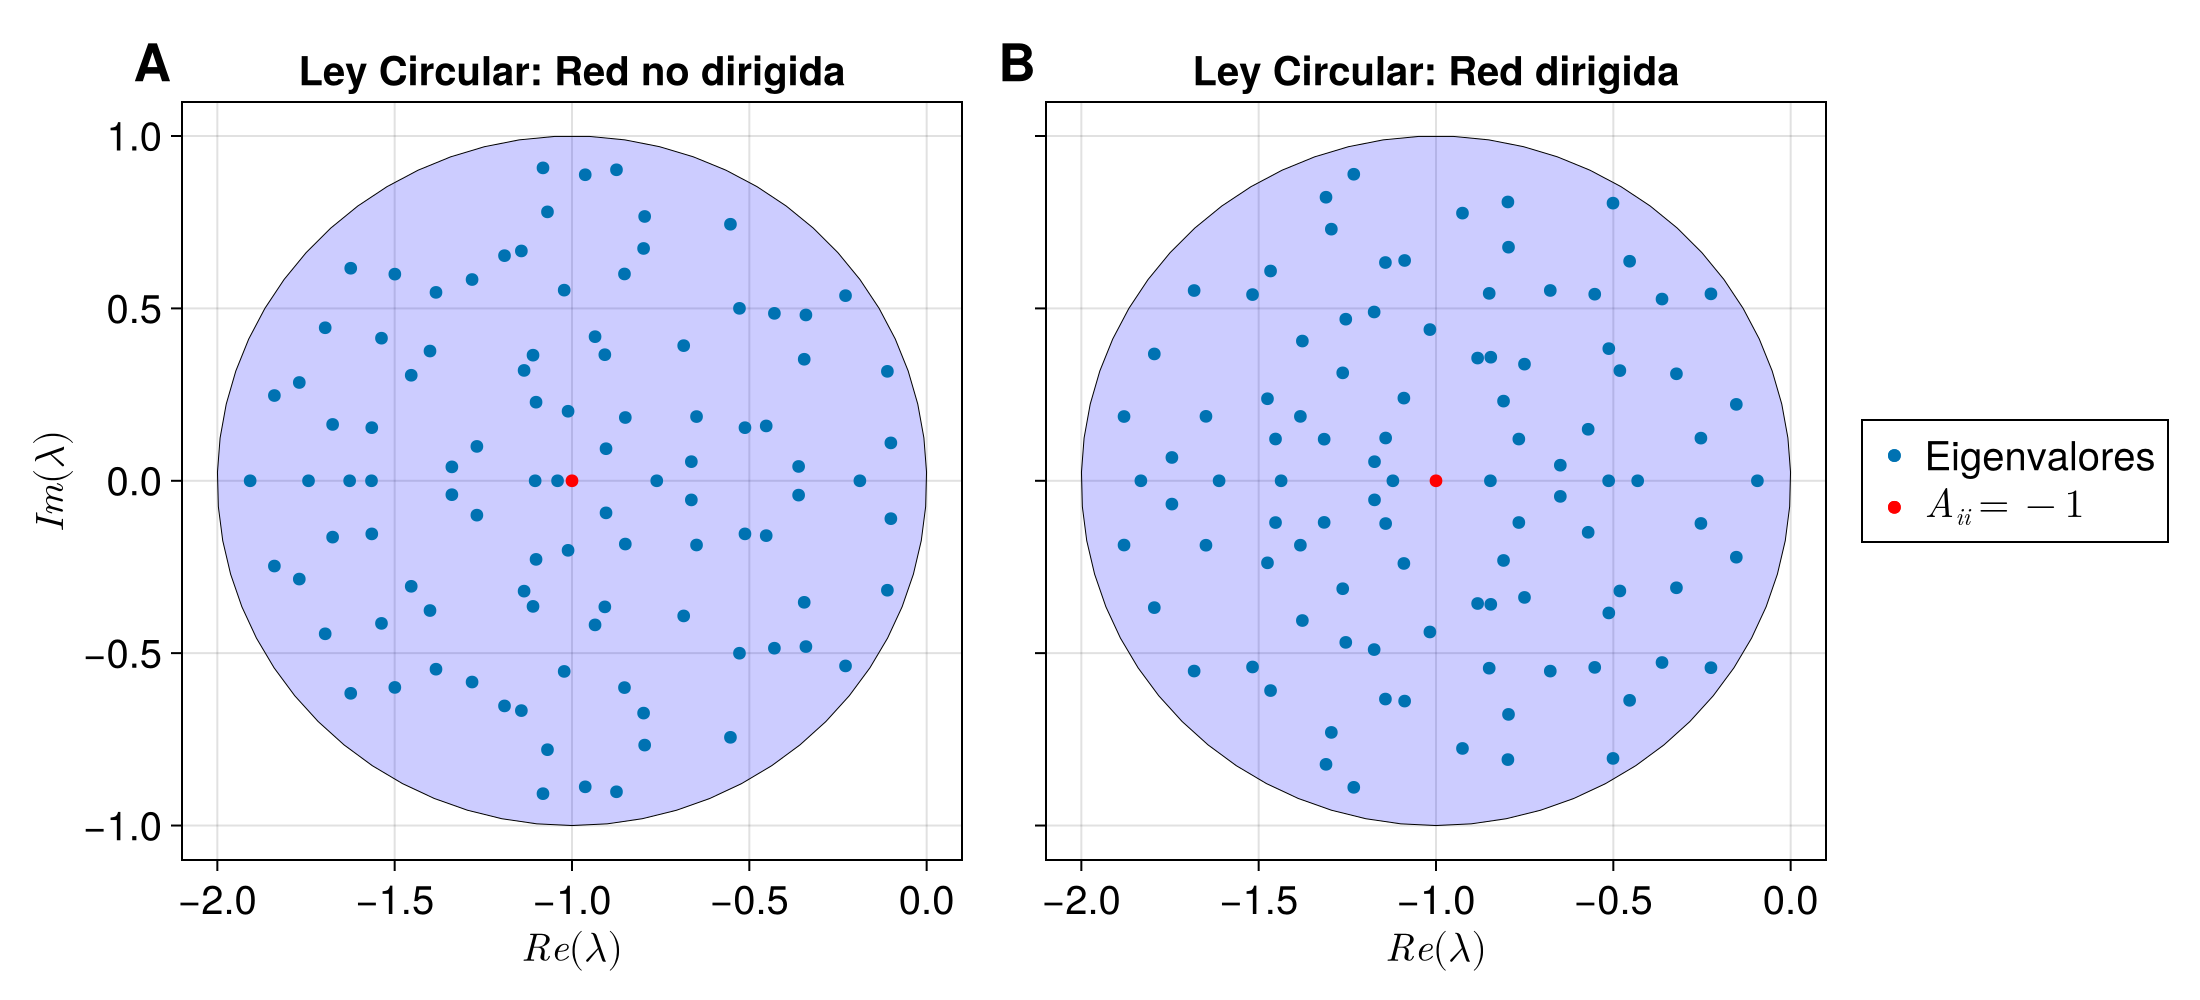
\includegraphics[scale=0.2]{../Imagenes/LeyCircularMay}
	\caption{Distribución de valores propios que cumplen la Ley Circular de May. Para ambos sistemas se consideró $N=100$, una distribución normal centrada en $\mu=0$ y con $\sigma=0.2$ para una conectancia $C=\frac{1}{\sigma^2 N}-0.03$. (\textbf{A}) Considerando una matriz de interacciones estructuralmente simétrica. (\textbf{B}) Considerando una matriz de interacciones puramente aleatoria.}
	\label{fig:LeyCircularMay}
\end{figure}

Cada sistema se ha considerado para $N=100$ especies ($A\in M_{100}(\mathbb{R})$), considerando una distribución normal centrada en $\mu=0$ con $\sigma=0.2$ y para una conectancia de $C=\frac{1}{\sigma^2 N}-0.03$. Si el sistema resultante no es estable entonces los valores propios se salen del confinamiento circular haciendo que algunos de ellos tengan parte real positiva. Para que esto ocurra se debe de considerar el contrario de la desigualdad (\ref{eqn:estabilidadMay}). 
\newpage
Para el sistema de Allesina \cite{allesina2012stability} se ha mencionado anteriormente que se consideran matrices de interacciones mapeadas a partir de una distribución bivariante. De esta forma nos permite realizar un cálculo de correlación $\rho$ entre ambas matrices triangulares de la matriz de interacciones. Al calcular la correlación entre ambas partes de la matriz de interacciones se define $a=1+\rho$ y $b=1-\rho$ como semi ejes de la elipse y dependiendo de como se encuentren los signos del resto de la matriz de interacciones es que se verán dos diferentes formas de distribución elíptica. Otro aspecto de esta matriz es que Allesina también consdiera a la diagonal fijada a un valor $A_{ii}= -d$ lo que implica que los valores propios estarán en la vecindad elíptica alrededor de $-d$.
\\
\\
La forma de la elipse, que podrá ser vertical u horizontal vendrá dada por el valor de la correlación, si se tienen interacciones ``presa-depredador'' $(+-)$ o $(-+)$ entonces la distribución elíptica resultante será vertical, en este caso habría que escoger una distribución normal con $\mu_1<0$ y otra con $\mu_2>0$. Por otro lado si las interacciones son de cooperación $(++)$ y/o competencia $(--)$ entonces la distribución elíptica será horizontal.
\begin{figure}[h!]
	\centering
	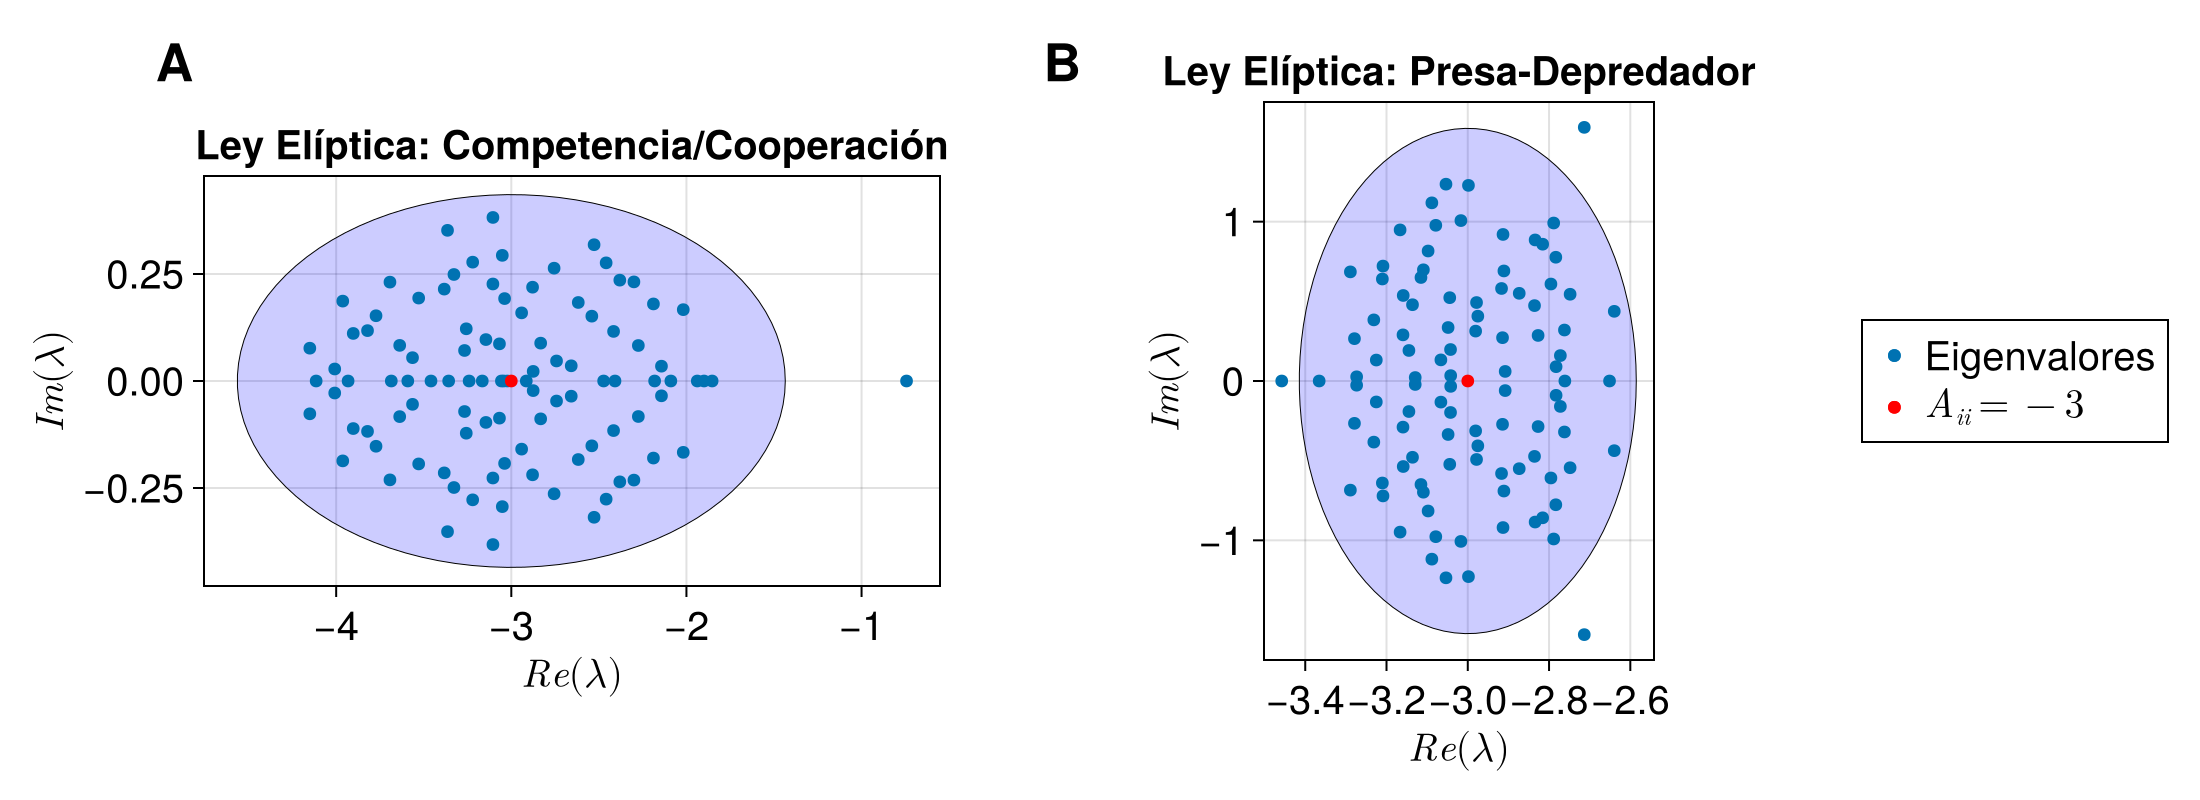
\includegraphics[scale=0.2]{../Imagenes/LeyElipticaAllesina}
	\caption{Ley Elíptica de Allesina. Ambos sistemas son de tamaño $N=100$. Se consideró una conectancia $C=0.12$ con matrices estructuralmente simétricas. (\textbf{A}) Considera una distribución normal con $\mu_1=0.1$ y $\sigma_1 = 0.1$ para la parte triangular superior y otra distribución normal con $\mu_2=0.3$ y $\sigma_2 = 0.2$ para la triangular inferior. (\textbf{B}) Considera una distribución con $\mu_1=-0.1$ y $\sigma_1=0.1$ para la parte triangular superior otra distribución normal con $\mu_2=0.3$ y $\sigma_2=0.2$ para la triangular inferior. }
	\label{fig:LeyElipticaAllesina}
\end{figure}

En la figura (\ref{fig:LeyElipticaAllesina}) se han considerado dos matrices de interacción, una con interacciones de competencia/cooperación y otra con interacciones presa depredador. Para que la distribución de valores propios pueda ajustarse a la elipse se deben de considerar matrices estructuralmente simétricas, ya que si fueran puramente aleatorias la correlación $\rho$ sería igual a cero y por lo tanto $a=b$ lo que daría lugar al resultado de May. El resultado de Allesina es interesante porque las interacciones ya poseen un sentido y estructura, no son independientes como en el caso de May. Si por ejemplo se tuviera $\rho>0$ implicaría que las especies tienden a cooperar o competir de forma similar. En contra parte, cuando $\rho <0$ entonces las especies tienden a un comportamiento presa-depredador. Por lo tanto los ejes capturan la forma de las interacciones dominantes del sistema. \\
\\
El fin de presentar estos resultados es para mostrar al lector las variantes que pueden existir en la estabilidad asumiendo diversas hipótesis en la construcción del sistema. Cada uno tiene su parámetro de transición de estabilidad y la misión de este trabajo es porponer una forma de acercarse al parámetro de transición del sistema de Lotka-Volterra generalizado, primordialmente cuando se consideran sistemas estructuralmente simétricos.

\subsection{Transición de May}

Una vez vista la distribución de valores propios de las matrices de May y Allesina, resta observar (únicamente para el caso de May) cómo cambia la estabilidad en función de la conectancia $C$ y la fuerza de interacción promedio $\sigma$. Se van a considerar matrices de May puramente aleatorias y se compararán con las que son estructuralmente simétricas, para observar si existen variaciones entre ambos casos. Se comenzará viendo la estabilidad en función de la conectancia $C$, considerando una familia distribuciones normales centradas en $\mu=0$ y con desviaciones estándar $\Sigma = \{0.1,0.2,...,1.0\}$. Todos los sistemas considerados en esta sección se harán para $N=100$. 
\begin{wrapfigure}{l}{0.5 \textwidth} \vspace{-30pt} \begin{center}
		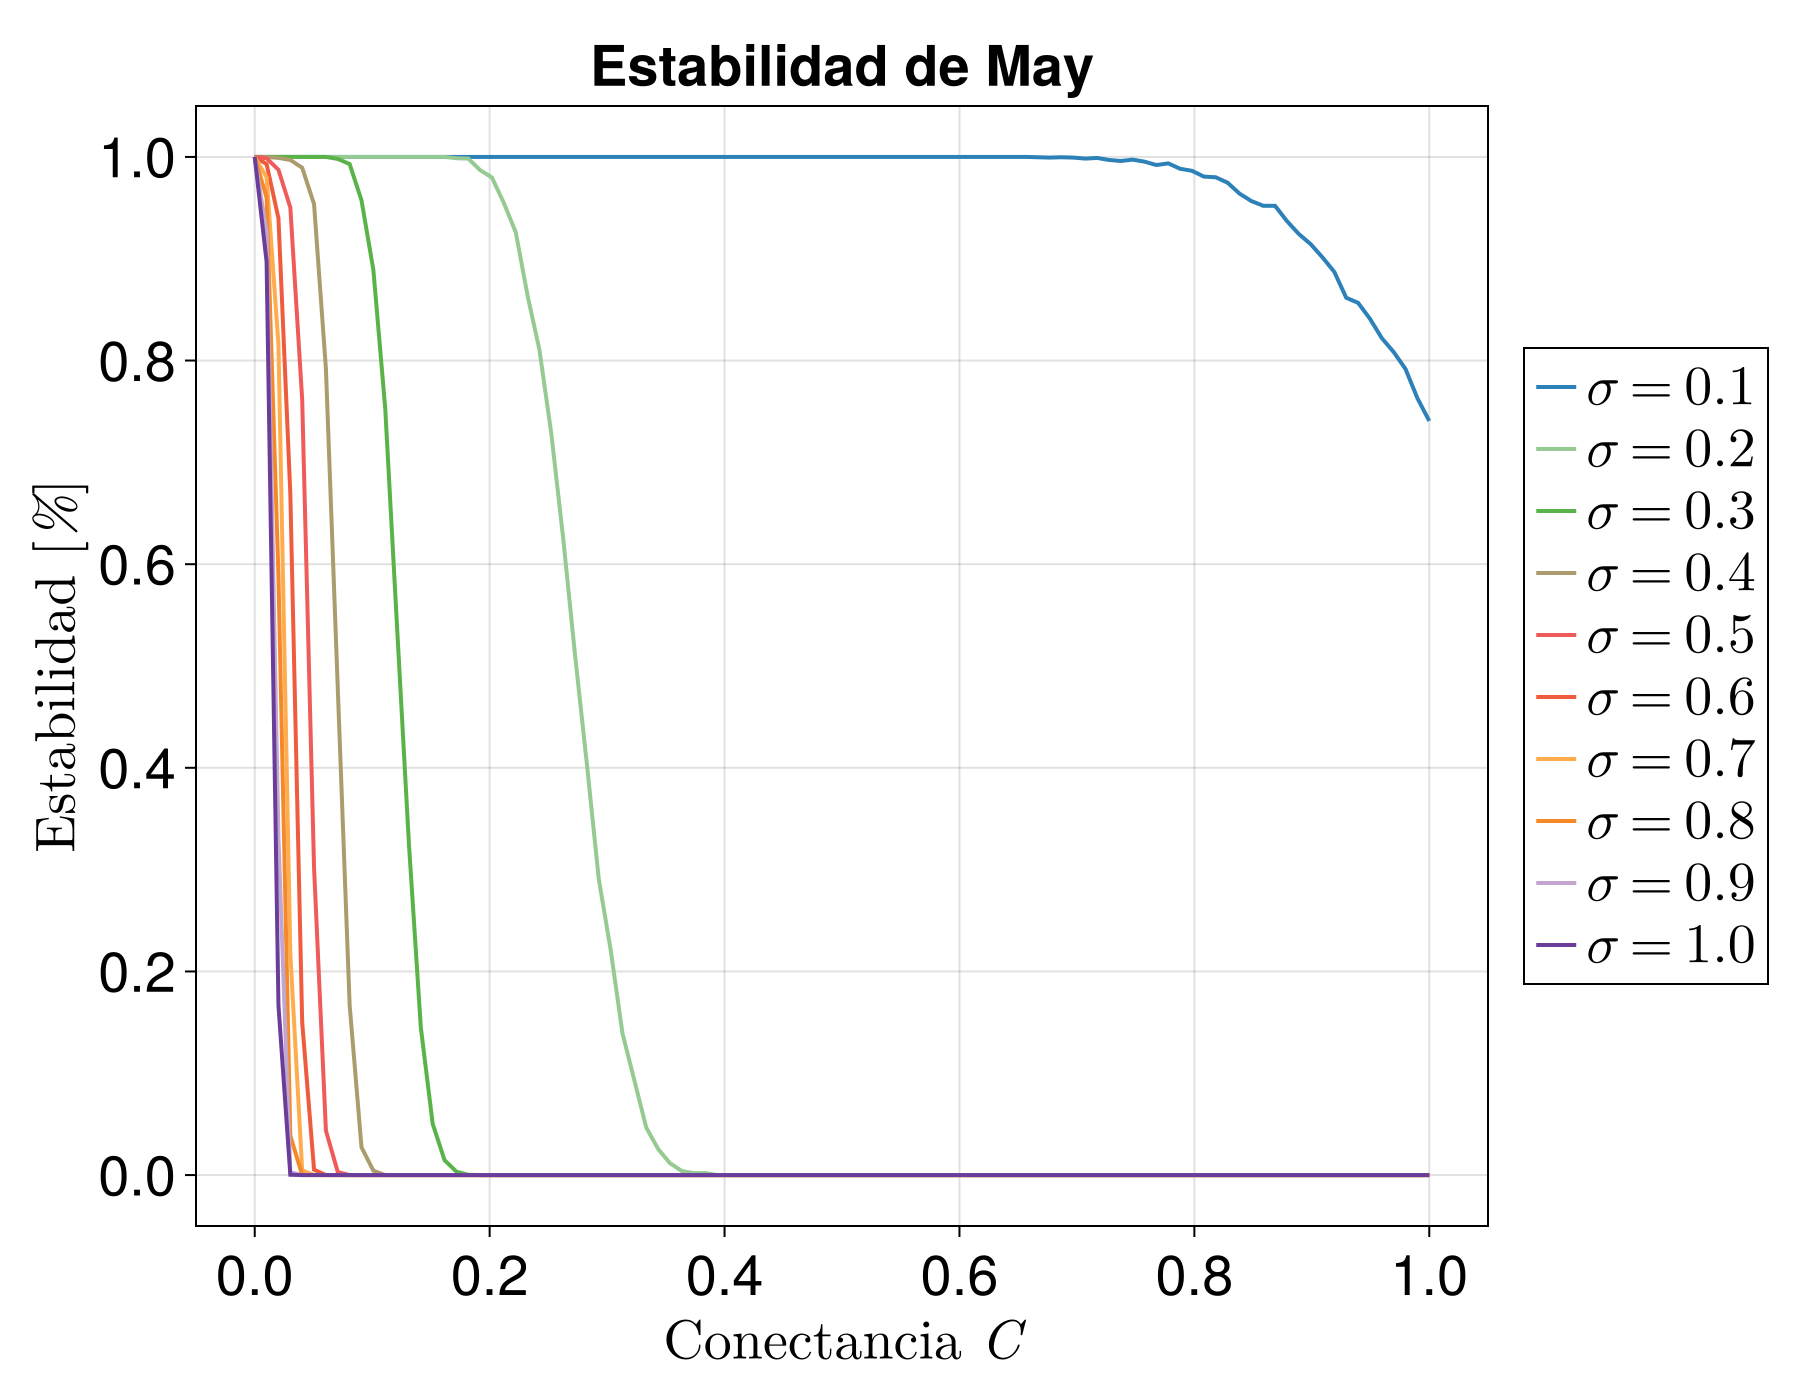
\includegraphics[width=0.52\textwidth]{../Imagenes/TransicionMayDirLin} 
	\end{center} 
	\vspace{-20pt} 
	\caption{Estabilidad de sistemas de May integrando para una partición equiespaciada de  $100$ conectancias en el intervalo $[0,1]$ y para una familia de distribuciones normales. Para cada valor de la conectancia se consideraron $3000$ simulaciones de las cuales se contabilizaron únicamente las estables con base en el signo de la parte real de sus valores propios.} 
	\vspace{-10pt}
	\label{fig:TransicionMayDirLin}
\end{wrapfigure} 
En cada uno de los diagramas de transición se van a contemplar $3000$ simulaciones por cada valor de $C$ o $\sigma$ (para $\sigma$ se verá más adelante) considerando para cada caso una partición equiespaciada de 100 valores entre 0 y 1. Se contabilizará el número de sistemas que resultaron ser estables con base en la parte real de sus valores propios. La figura (\ref{fig:TransicionMayDirLin}) muestra el cambio de estabilidad en función de la conectancia y para la familia de distribuciones normales con sus respectivas desviaciones estándar provenientes de $\Sigma$. Se aprecia que a medida que la fuerza de las interacciones aumenta es cada vez menos probable que sea estable, obedeciendo como tal al parámetro (\ref{eqn:radioMayGirko}). Convendría realizar un acercamiento para observar la transición para los valores $\sigma>0.3$, misma que se puede hacer considerando valores de escala $\log_{10}$.\\
\\
Al aplicar el re-escalamiento se podrán apreciar mejor las transiciones para valores  $\sigma\geq3$ de la fuerza promedio. En este caso se verá como dichas transiciones ocurren para valores de la conectancia entre $10^{-2}$ hasta $10^{-1}$ ajustándose a lo que dicta el parámetro (\ref{eqn:radioMayGirko}). La ventaja de que los sistemas de May consideren las diagonales fijas en $A_{ii}=-1$ para toda $A_{ii}\in A$ es que la transición se percibe muy marcada, pues justamente en $CN\sigma^2=1$ se tiene el disco de Gershgorin más grande en el semiplano
\begin{wrapfigure}{r}{0.5 \textwidth} \vspace{-30pt} \begin{center}
		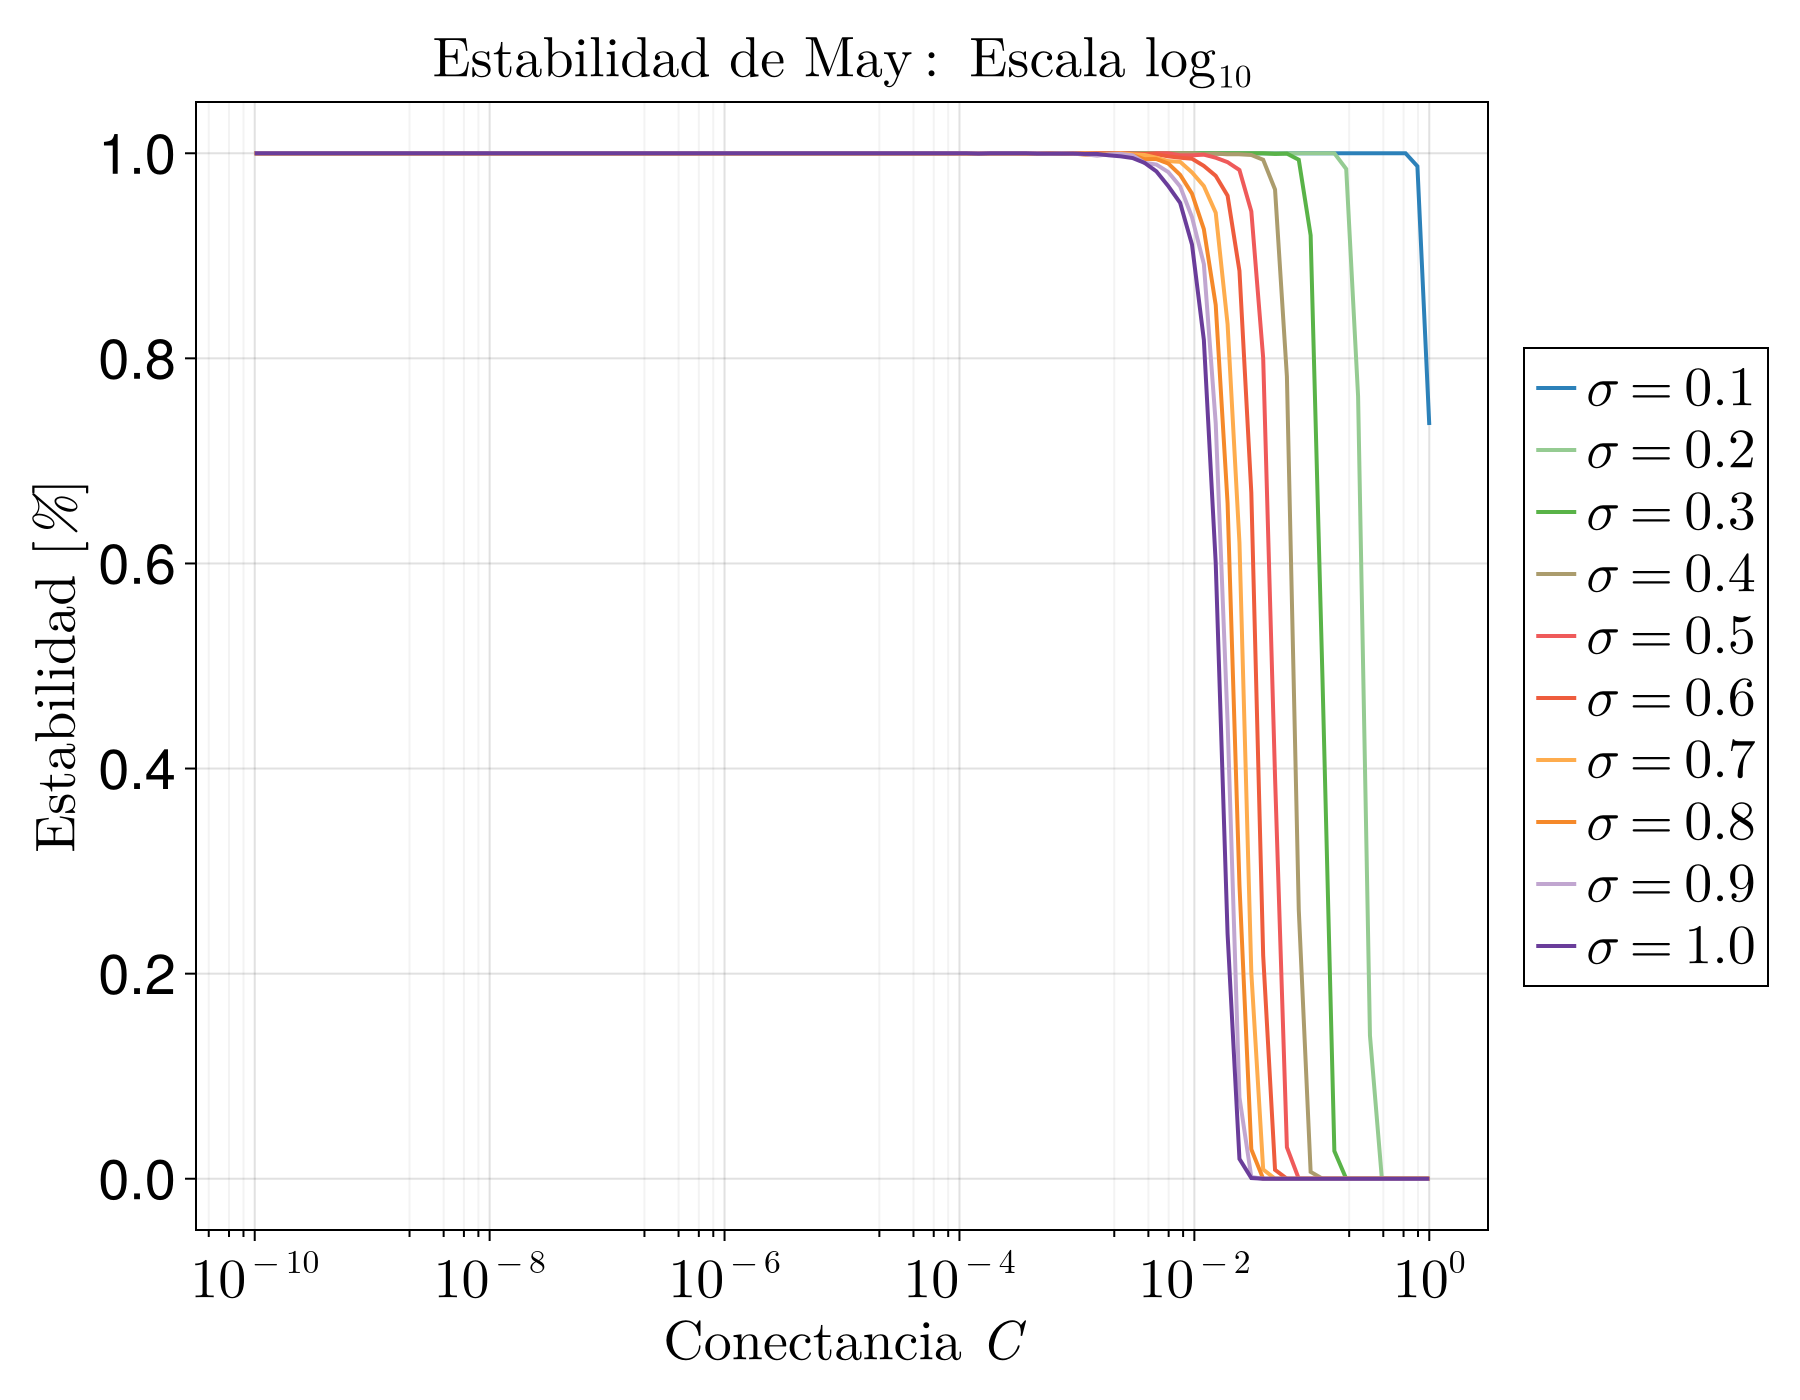
\includegraphics[width=0.52\textwidth]{../Imagenes/TransicionMayDirLog} 
	\end{center} 
	\vspace{-20pt} 
	\caption{Estabilidad de May de la figura (\ref{fig:TransicionMayDirLin}) en función de $C$ con escala $\log_{10}$.} 
	\vspace{-10pt}
	\label{fig:TransicionMayDirLog}
\end{wrapfigure} 

negativo de $\mathbb{C}$ que coincide con la Ley Circular de May, y a partir de ahí, para $CN\sigma^2>1$ los discos comienzan a ser más grandes pudiendo alojar valores propios con parte real positiva. Desde ahora es válido preguntarse como sería la transición cuando la diagonal de la matriz no es homogénea, se irá abordando en el siguiente capítulo. Actualmente se han considerado únicamente matrices de May puramente aleatorias; al compararlas con sistemas de May estructuralmente simétricos la estabilidad cambia y es lo que se verá a continuación. Los cambios son notorios para cada valor de $\Sigma$ pero es más pronunciado cuanto mayor es $\sigma$. Se visualizarán las diferencias para los casos $\sigma= 0.2$ y $\sigma = 0.6$
\begin{figure}[h!]
	\centering
	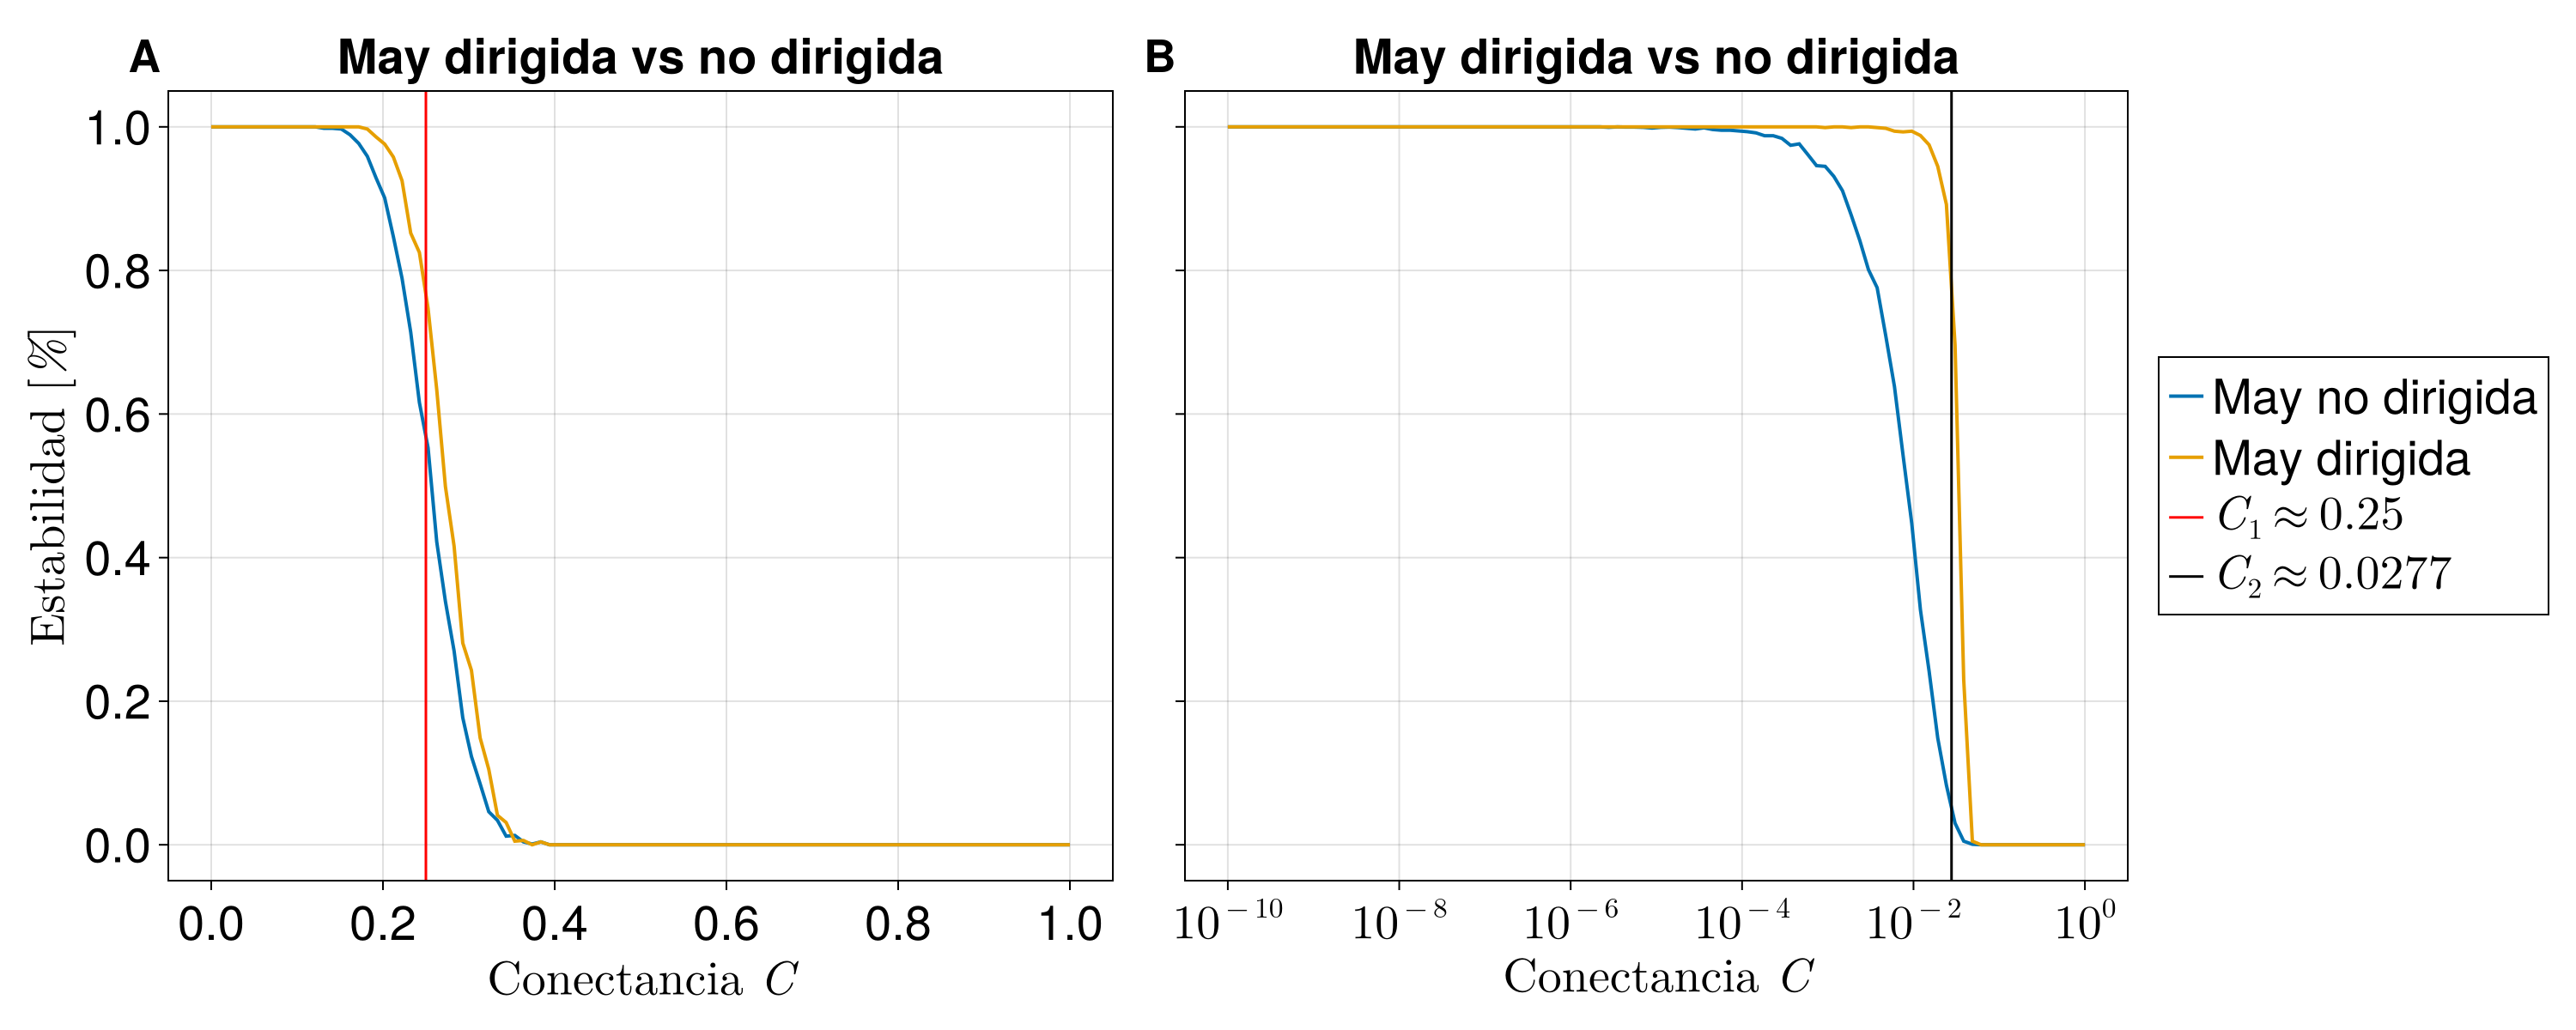
\includegraphics[scale = 0.165]{../Imagenes/TransicionDirvsNoDir}
	\caption{Transición de May puramente aleatoria vs estructuralmente simétrica. (\textbf{A}) Se considera para $\sigma = 0.2$ (\textbf{B}) Se considera para $\sigma=0.6$.}
	\label{fig:TransicionDirvsNoDir}
\end{figure}
en la figura (\ref{fig:TransicionDirvsNoDir}) y percibiendo que el parámetro de transición (\ref{eqn:radioMayGirko}) se ajusta correctamente a las matrices de May puramente aleatorias pero no hace lo mismo para los sistemas estructuralmente simétricos, lo que sugiere que debe de existir algún otro elemento determinante en la estabilidad que tiene que ver con la simetría de las interacciones y con el valor de $\sigma$.
\\
\\
Para el caso de la transición en función de $\sigma$ se tiene un resultado similar. Ahora se consideró la familia de conectancias $\tilde{C}=\{0.1,0.2,...,1.0\}$ y la partición equiespaciada de $\sigma$ con 100 valores entre 0 y 1. La tendencia de la estabilidad igual obedece al parámetro de May (\ref{eqn:radioMayGirko}) aunque de forma distinta pues, el valor crítico $\sigma^*$ es proporcional a $\frac{1}{\sqrt{N}}$ y $C^*\propto \frac{1}{N}$, entonces $\sigma^*>C^*$, y por lo tanto las transiciones en función de $\sigma$ ocurren más hacia la derecha. 
\begin{figure}[h!]
	\centering
	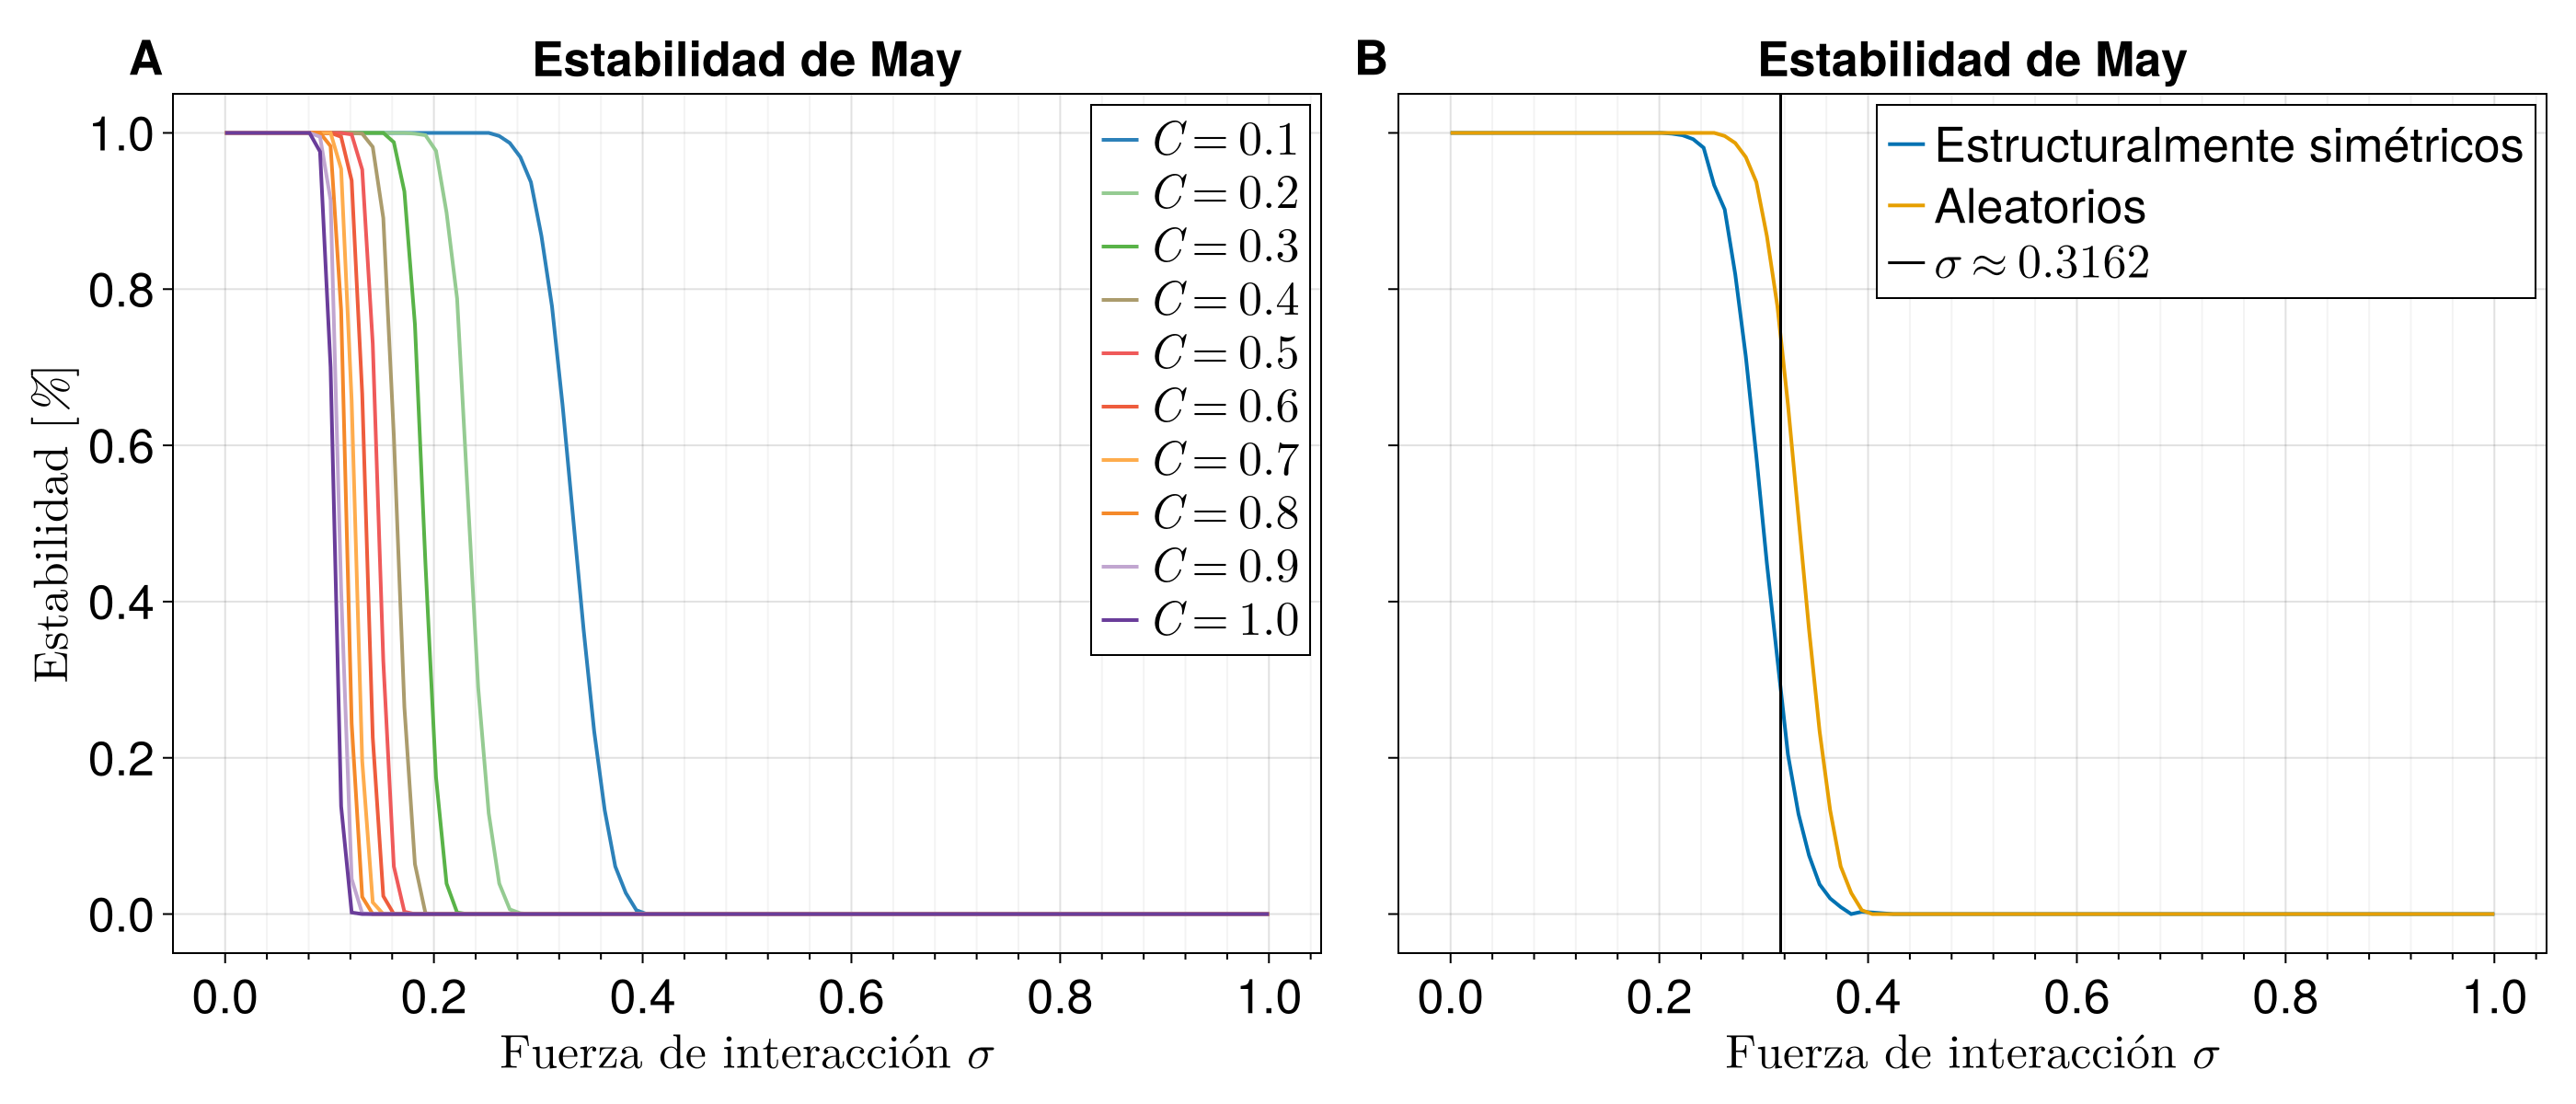
\includegraphics[scale = 0.165]{../Imagenes/TransicionMaySigma}
	\caption{Transición de estabilidad en función de $\sigma$ (\textbf{A}) Se considera para una familia de conectancias $\tilde{C}$ y una partición equiespaciada de 100 valores de $\sigma$ entre 0 y 1. Se consideran 3000 simulaciones por cada valor de $\sigma$ y se contabilizan los sistemas estables con base en la parte real de los valores propios de cada simulación. (\textbf{B}) Caso particular para $C=0.1$; se consideran las diferencias entre la matriz de May estructuralmente simétrica y la matriz puramente aleatoria.}
	\label{fig:TransicionMaySigma}
\end{figure}
Algo importante a notar es que aún con el valor de la conectancia $C=0.1$, a medida que $\sigma$ aumenta los sistemas son cada vez menos estables, a diferencia de la transición en función de $C$ que para $\sigma=0.1$ no se observaba un cambio abrupto en la estabilidad (Fig. (\ref{fig:TransicionMayDirLin})). Esto podría implicar que la fuerza de las interacciones tiene mayor peso que la misma conectividad de la red, lo cual tiene sentido si se considera que en (\ref{eqn:radioMayGirko}) se encuentra el cuadrado de $\sigma$, que impone más peso sobre $C$. Lo importante de estos diagramas de transición es observar como cambia la estabilidad cuando una de las cantidades ($\sigma$ ó $C$) se mantiene fija y la otra variable. Los diagramas nos brindan información que será útil para tomar de referencia en las transiciones de estabilidad del sistema de Lokta-Volterra generalizado.\\
\\
En la Figura (\ref{fig:TransicionMaySigma} \textbf{B}) se observa la diferencia de estabilidad entre sistemas de May puramente aleatorios y estructuralmente simétricos para $C=0.1$. La desviación que presenta para este caso particular es considerablemente mayor si se compara con los sistemas que tienen conectancia $C=0.6$ tal y como se observa en la Figura (\ref{fig:TransicionσDirvsNoDir}).
\newpage
\begin{wrapfigure}{l}{0.5 \textwidth} \vspace{-30pt} \begin{center}
		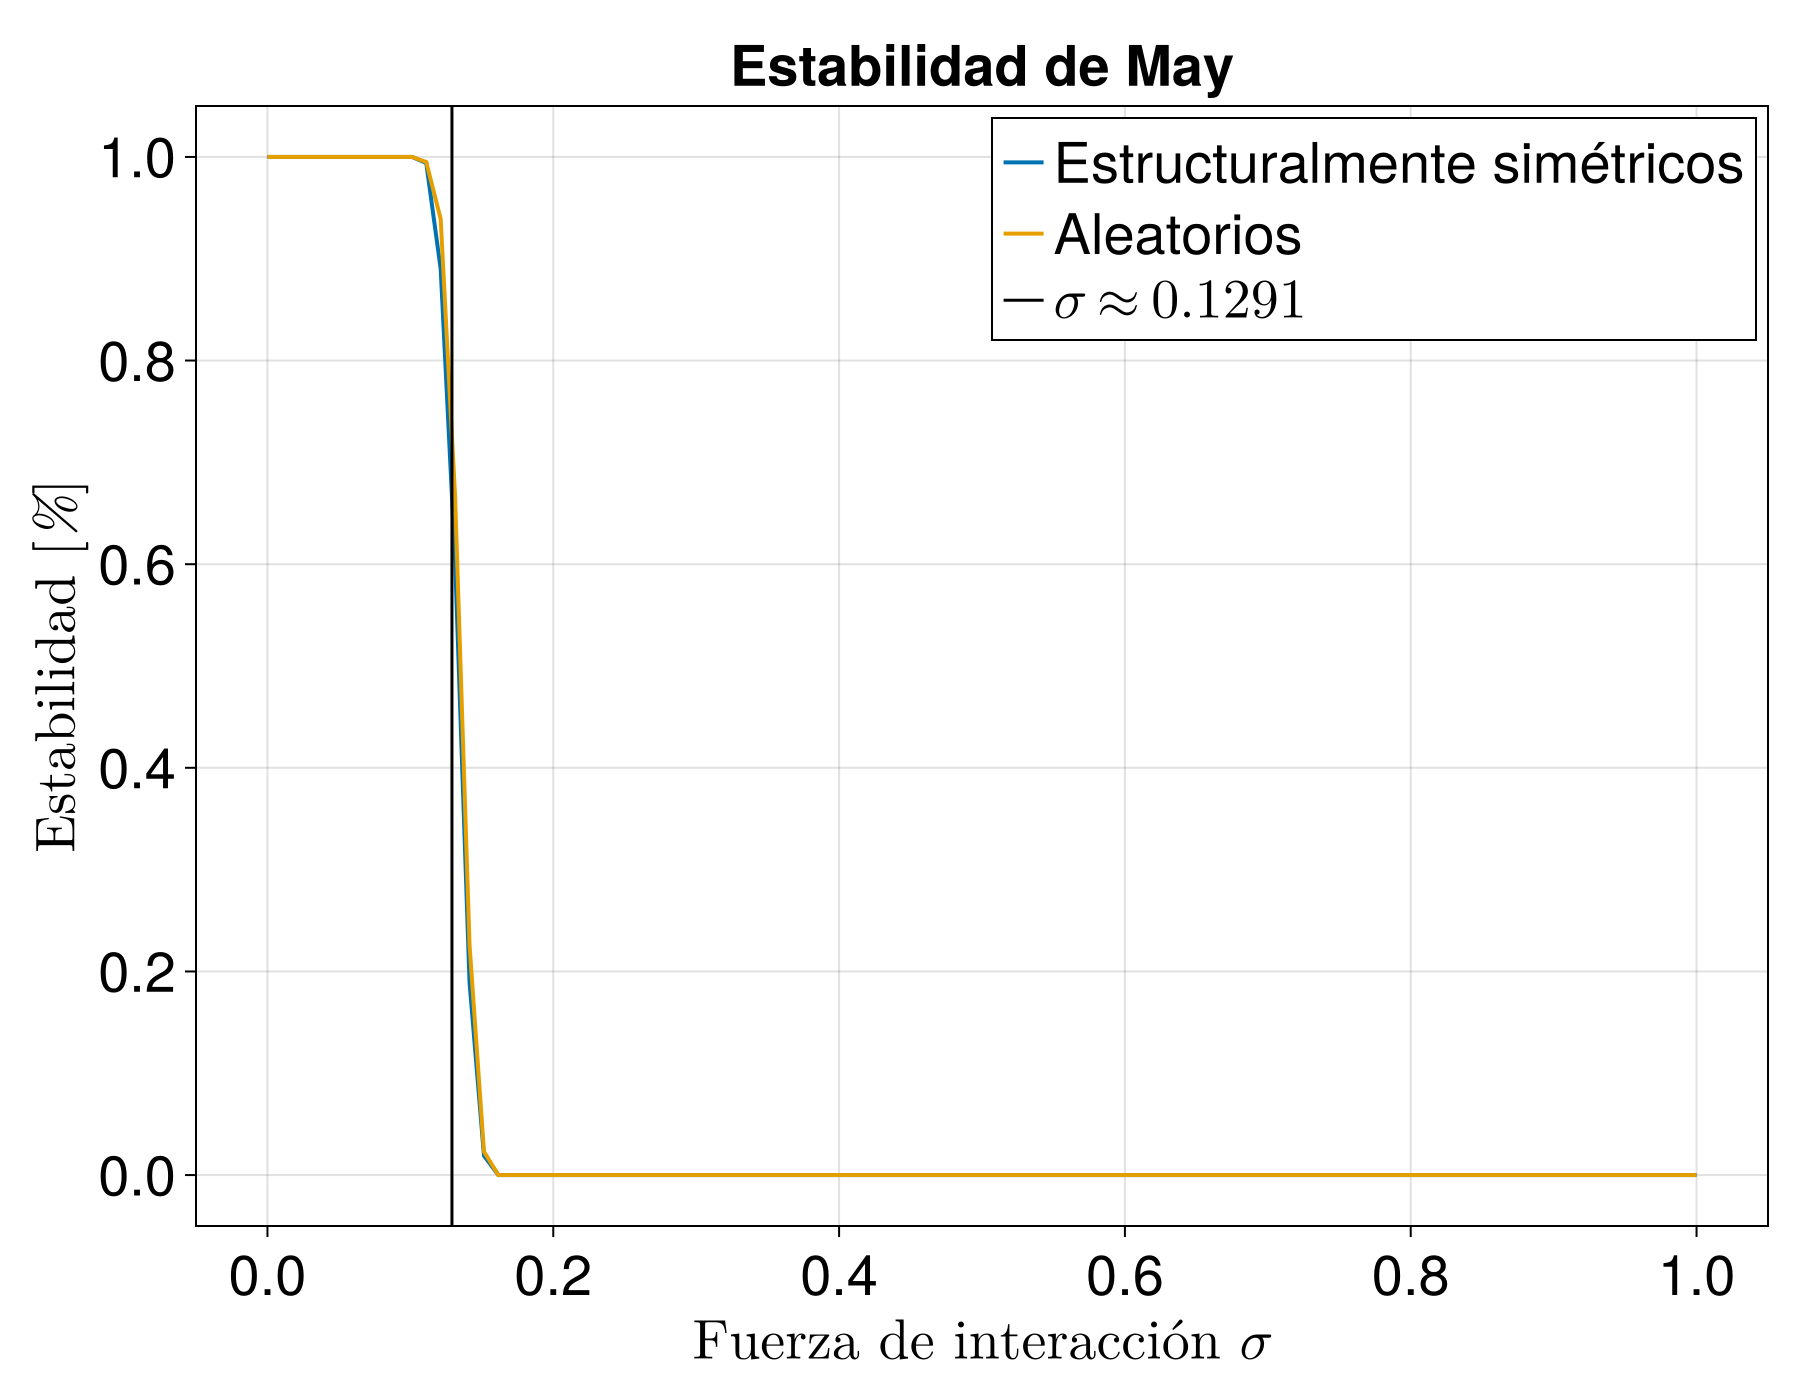
\includegraphics[width=0.52\textwidth]{../Imagenes/TransicionσDirvsNoDir} 
	\end{center} 
	\vspace{-20pt} 
	\caption{Variaciones en la transición de estabilidad para la matriz de May estructuralmente simétrica y para matriz puramente aleatoria. Se consideró el valor de la conectancia $C=0.6$.} 
	\vspace{-10pt}
	\label{fig:TransicionσDirvsNoDir}
\end{wrapfigure} 
A diferencia de las transiciones en función de la conectancia, cuanto mayor sea la $C$ se observa que las variaciones son prácticamente nulas entre los sistemas aleatorios y estructuralmente simétricos y son más notorias para valores de $C$ cercanos a cero. Esto induce a nuevas pistas sobre la naturaleza de transición de los sistemas estructuralmente simétricos, en términos de como es su relación con $C$ y $\sigma$. Lo que se puede asegurar con base en este breve esbozo es que la estabilidad depende de otros elementos que se podrían agregar al parámetro de May o que bien podrían ser completamente distintos de lo que se tiene concebido hasta ahora.\\
\\
Para cerrar con esta sección y capítulo, se va a mostrar una comparativa entre diagramas de transición de May en función de $\sigma$ y de $C$ con parámetros similares. Para ello se realizará un re-escalamiento del eje $x$ para ponerlo en función de $\sigma\sqrt{NC}$ con $C$ o $\sigma$ variando según sea el caso. Al realizar esto se verá que el parámetro de transición se ajusta a $1$, valor correspondiente a la diagonal de las matrices de los sistemas (y al radio máximo de discos de Gershgorin para alojar valores propios con parte real negativa). A continuación se muestran un par de escenarios para visualizar dicha comparativa.
\begin{figure}[h!]
	\centering
	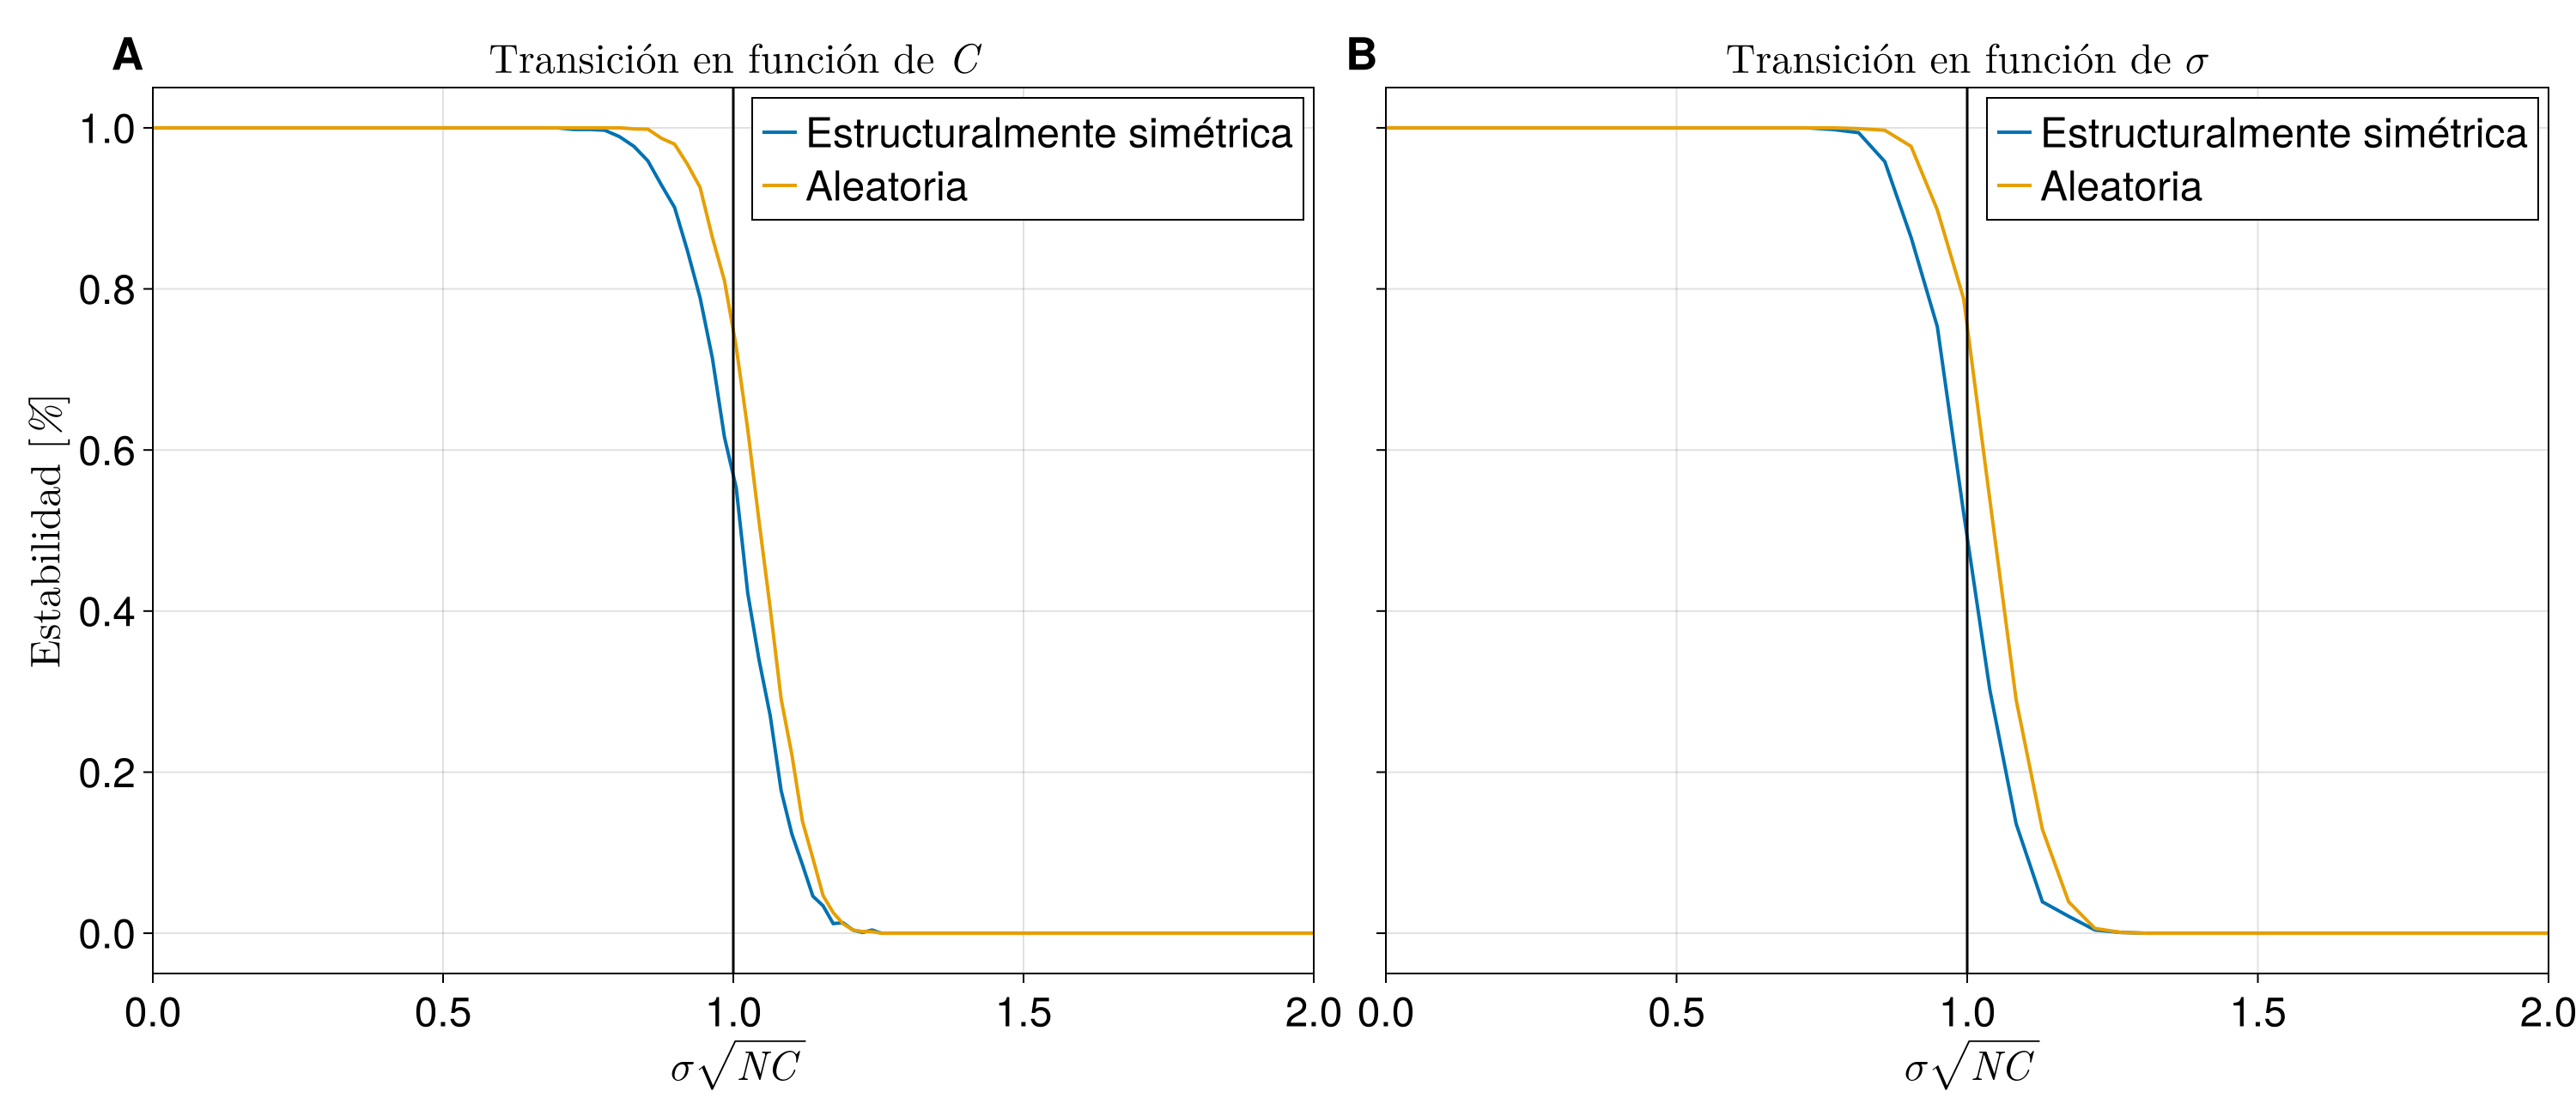
\includegraphics[scale=0.160]{../Imagenes/Transicionσ√NC02}
	\caption{Re-escalamiento del eje $x$ para visualizar las transiciones de la conectancia $C$ y la fuerza promedio de las interacciones $\sigma$. Para este caso particular se escogió $\sigma=C=0.2$. Se consideran sistemas de May aleatorios y estructuralmente simétricos.}
	\label{fig:Transicionσ√NC02}
\end{figure}

En la Figura (\ref{fig:Transicionσ√NC02}) se puede notar una gran compatibilidad para los valores $C_1=\sigma_1=0.2$, ya que $\sigma$ es lo suficientemente chico en (\textbf{A}) para generar poca desviación, y por el contrario para (\textbf{B}) la $C$ es suficientemente chica para generar gran desviación. Esto contrasta completamente con el segundo caso de la Figura (\ref{fig:Transicionσ√NC06}) para $C_2=\sigma_2=0.6$ en donde se percibe una gran desviación en (\textbf{A}) debido a que $\sigma$ ha aumentado su valor mientras que en su caso homólogo (\textbf{B}) se ajusta cada vez más a las matrices de May puramente aleatorias a medida que $C$ va aumentando. De la Figura (\ref{fig:Transicionσ√NC06} \textbf{A}) se puede notar el gran peso que ejerce la fuerza promedio de las interacciones, pues independientemente de la $C$ que le toque ya existe un gran porcentaje de sistemas inestables que emergen mucho antes del parámetro de transición de May.
\begin{figure}[h!]
	\centering
	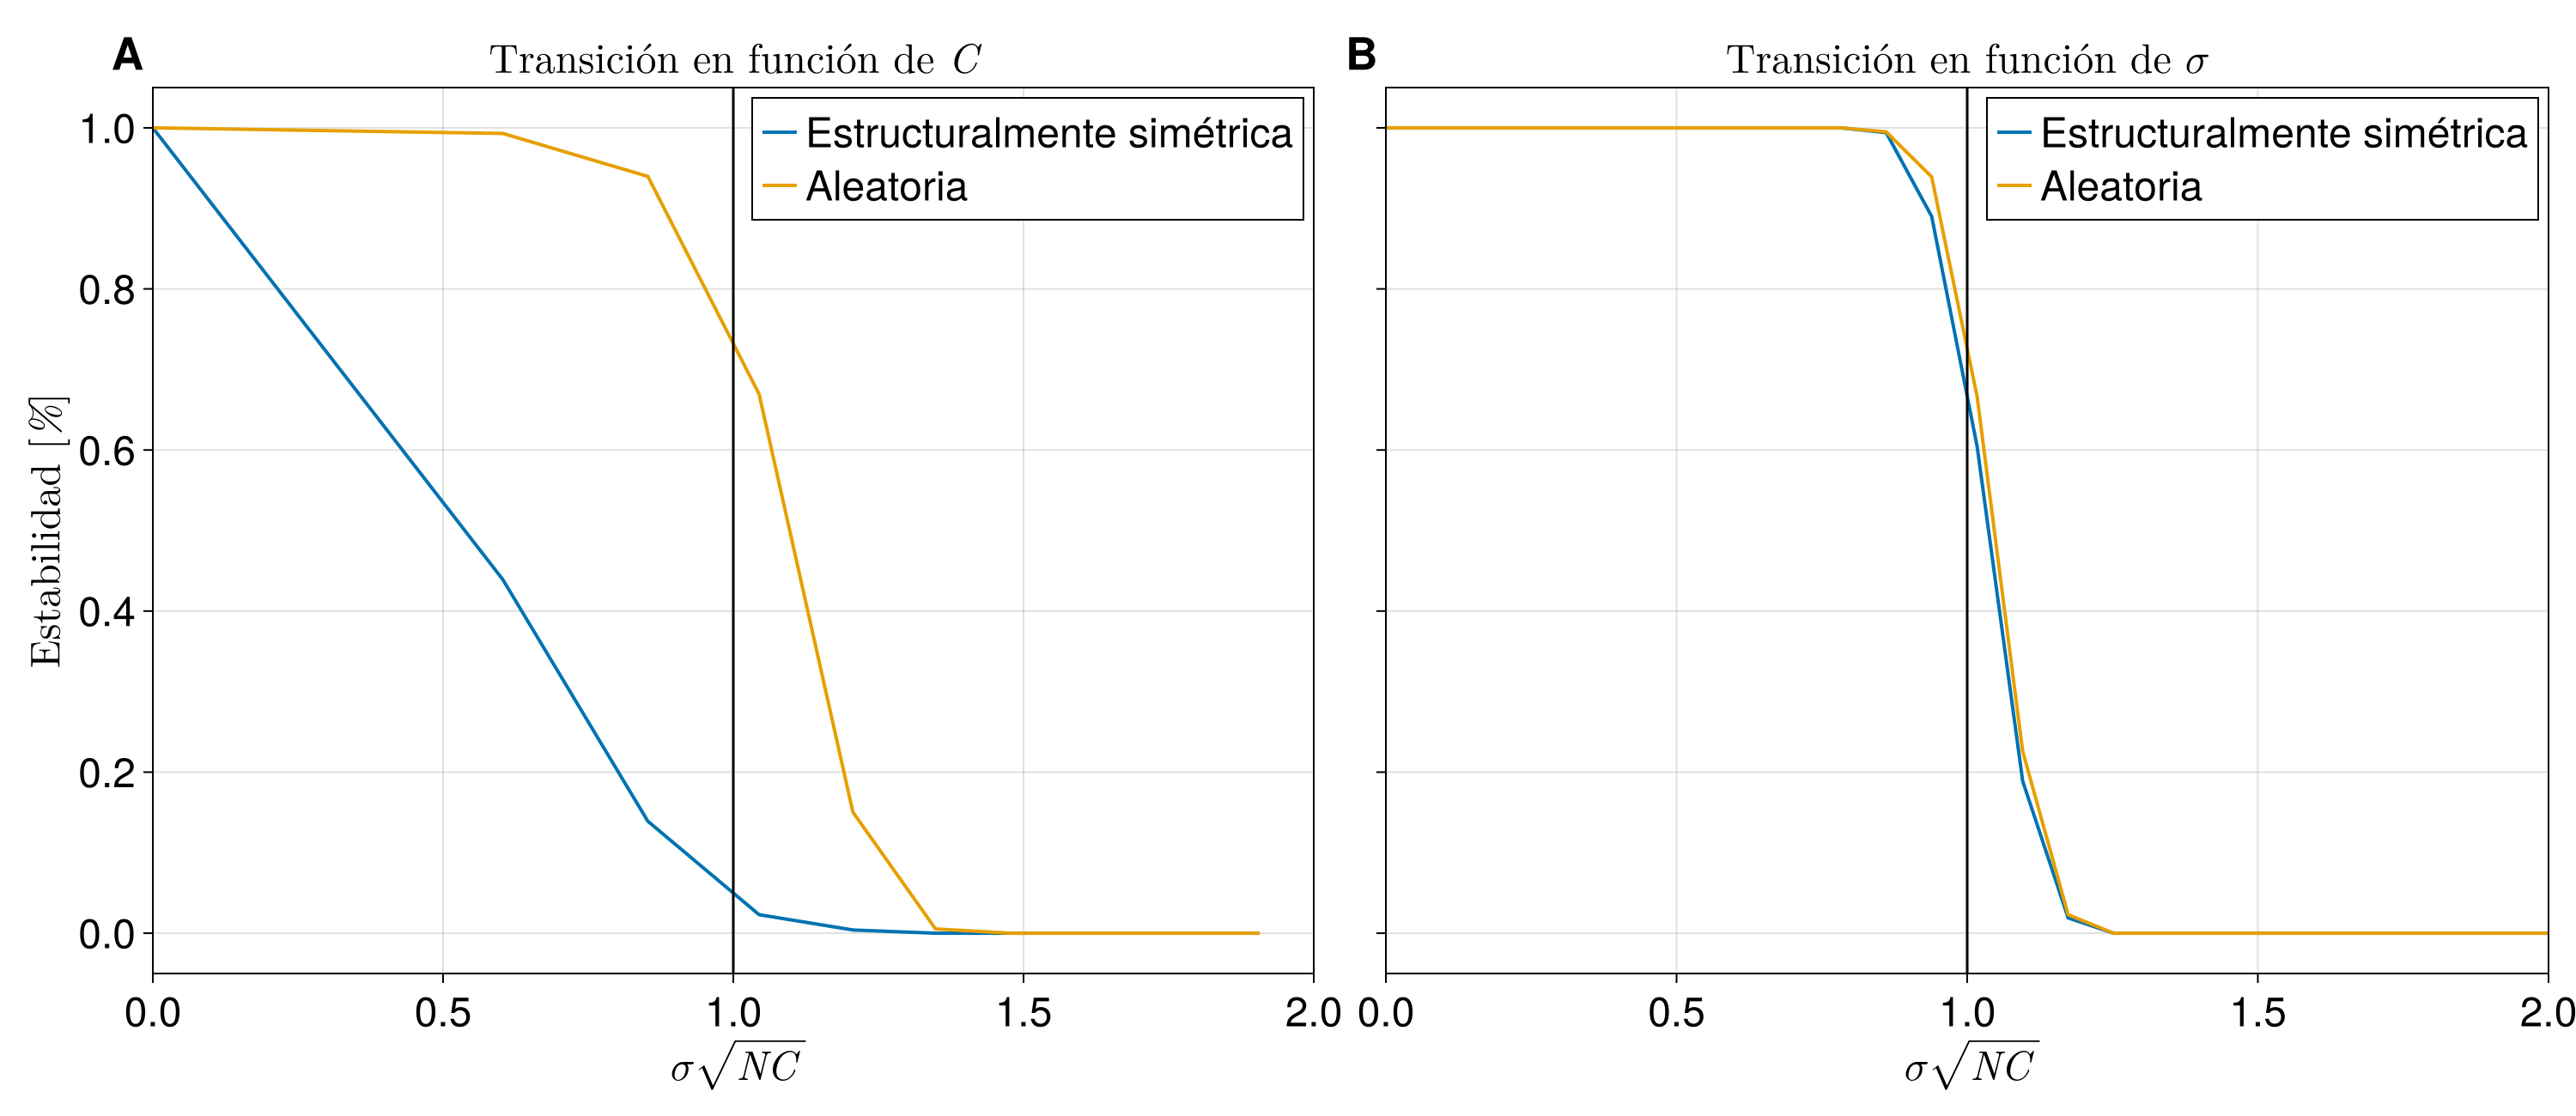
\includegraphics[scale=0.160]{../Imagenes/Transicionσ√NC06}
	\caption{Re-escalamiento del eje $x$ para visualizar las transiciones de la conectancia $C$ y la fuerza promedio de las interacciones $\sigma$. Para este caso particular se escogió $\sigma=C=0.6$. A diferencia del  caso anterior, se logra apreciar la desviación que ocurre en (\textbf{A}) cuando $\sigma$ se va acercando a 1.0.}
	\label{fig:Transicionσ√NC06}
\end{figure}




%Esta última sección está motivada para que el lector se dé una idea de lo que iremos a explorar con los resultados del siguiente capítulo. Se tiene en primera instancia lo de la distribución de eigenvalores pero también se pretenderá explorar el parámetro crítico que demarca las condiciones de estabilidad e inestabilidad para los sistemas.


%Estos elementos son claves para que podamos concebir la estabilidad para el sistema que hemos creado hasta ahora. Se tienen diferencias muy marcadas, nuestra matriz de interacciones $\mathcal{I}$ y la matriz de interacciones de May $A$: difícilmente tendrá su diagonal en $-1$ tal como $A$, sobre todo si se considera un sistema $n\gg 1$ especies. Esto genera un impacto en la distribución de los eigenvalores en el espacio complejo sin embargo al final de cuentas es estabilidad. Por esta misma razón, el parámetro de May (\ref{eqn:parametroMay}) puede no ajustarse perfectamente con nuestros resultados.